% Präambel
\documentclass[11pt,a4paper,oneside, 
liststotoc, 					% Tabellen- und Abbildungsverzeichnis ins Inhaltsverzeichnis
bibtotoc,						% Literaturverzeichnis ins Inhaltsverzeichnis aufnehmen
titlepage, 						% Titlepage-Umgebung statt \maketitle
headsepline, 					% horizontale Linie unter Kolumnentitel
%abstracton,					% Überschrift beim Abstract einschalten, Abstract muss dazu in {abstract}-Umgebung stehen
%DIV11,							% auskommentieren, um den Seitenspiegel zu vergrößern
BCOR6mm,						% Bindekorrektur, die den Seitenspiegel um 6mm nach rechts verschiebt,
]{scrreprt}			
\usepackage{ucs} 				% Dokument in utf8-Codierung schreiben und speichern
\usepackage[utf8x]{inputenc} 	% ermöglicht die direkte Eingabe von Umlauten
\usepackage[english]{babel} 	% deutsche Trennungsregeln und Übersetzung der festcodierten Überschriften
\usepackage[T1]{fontenc} 		% Ausgabe aller zeichen in einer T1-Codierung (wichtig für die Ausgabe von Umlauten!)
\usepackage{graphicx}  			% Einbinden von Grafiken erlauben
%\usepackage{amsmath}
%\usepackage{amsfonts}
%\usepackage{amssymb}
\usepackage{mathpazo} 			% Einstellung der verwendeten Schriftarten
\usepackage{textcomp} 			% zum Einsatz von Eurozeichen u. a. Symbolen
\usepackage{listings}			% Datstellung von Quellcode mit den Umgebungen {lstlisting}, \lstinline und \lstinputlisting
\usepackage{xcolor} 			% einfache Verwendung von Farben in nahezu allen Farbmodellen
\usepackage[intoc]{nomencl} 	% zur Erstellung des Abkürzungsberzeichnisses
\usepackage{fancyhdr}			% Zusatzpaket zur Gestaltung von Fuß und Kopfzeilen
\usepackage{listing}
\usepackage{setspace}
\usepackage{nameref}

% -----------------------------------------------------------------------------------------------------------------
% Zum Aktualisieren des Abkürzungsverzeichnisses bitte auf der Kommandozeile folgenden Befehl aufrufen :
%  makeindex Bachelorarbeit.nlo -s nomencl.ist -o Bachelorarbeit.nls
% -----------------------------------------------------------------------------------------------------------------

% Hier die persönlichen Daten eingeben:

\newcommand{\titel}{Assistenzsystem für Quadrocopter}
\newcommand{\untertitel}{}
\newcommand{\arbeit}{Studienarbeit}
\newcommand{\studiengang}{Angewandte Informatik}
\newcommand{\autor}{Christoph Meise}
\newcommand{\matrikelnr}{4050853}
\newcommand{\kurs}{TINF14B2}
\newcommand{\firma}{SAP SE}
\newcommand{\abgabe}{09.19.2016}
\newcommand{\betreuerdhbw}{Markus Strand}\newcommand{\betreuerfirma}{Andreas Wendel}

\newcommand{\jahr}{2016}			% für Angabe im Copyright-Vermerk der Titelseite

% Abkürzungen
\newcommand{\ua}{\mbox{u.\,a.\ }}
\newcommand{\zB}{\mbox{z.\,B.\ }}
\newcommand{\bs}{$\backslash$}

\renewcommand{\nomname}{List of Abbreviations}

% -------------------------------------------------------------------------------------------
% Definition der Kopf- und Fußzeilen
\lhead{}								% Kopf links
\chead{}								% Kopf mitte
\rhead{\sffamily{\titel}}				% Kopf rechts
\lfoot{}								% Fuß links
\cfoot{\sffamily{\thepage}}				% Fuß mitte
\rfoot{\sffamily{\autor}}				% Fuß rechts
\renewcommand{\headrulewidth}{0.4pt}	% Liniendicke Kopf
\renewcommand{\footrulewidth}{0.4pt}	% Liniendicke Fuß

\makeatletter
\newcommand*{\currentname}{\@currentlabelname}
\makeatother



\makenomenclature							% Abkürzungsverzeichnis erstellen

% alle Abkürzungen, die in der Bachelorarbeit verwendet werden

\nomenclature{IoT}{Internet of Things}








					% Datei mit Abkürzungen laden

% -------------------------------------------------------------------------------------------
%                     Beginn des Dokumenteninhalts
% -------------------------------------------------------------------------------------------
\begin{document}
\begin{spacing}{1.5}
\setcounter{secnumdepth}{3}					% Nummerierungstiefe fürs Inhaltsverzeichnis
\setcounter{tocdepth}{3}
\sffamily									% für die Titelei serifenlose Schrift verwenden

% ------------------------------ Titelei -----------------------------------------------------

\thispagestyle{plain}
\begin{titlepage}
\begin{spacing}{1.0}
\enlargethispage{4.0cm}
\sffamily 								% Serifenlose Grundschrift für die Titelseite einstellen
				
\begin{figure}
\begin{minipage}[htbp]{5cm}
	\centering
	
\includegraphics[scale=0.25]{Bilder/522x294.jpg}

	%\label{Bild1}
\end{minipage}
\hfill
\begin{minipage}[htbp]{5cm}
	\centering 
	
\includegraphics[scale=2.0]{Bilder/logo_dhbw.jpg}

	%\label{Bild2} 
\end{minipage} 
\end{figure}

% \begin{flushleft}
% 
\includegraphics[scale=0.35]{Bilder/522x294.jpg}\\[0ex]
% \end{flushleft}
% 				
% \begin{flushright}
% 
\includegraphics[scale=2.0]{Bilder/logo_dhbw.jpg}\\[0ex]
% \end{flushright}

\begin{center}

\huge{\textsc{\textbf{\titel}}}\\[1.5ex]
\Large{\textbf{\untertitel}}\\[5ex]
\LARGE{\textbf{\arbeit}}\\[2ex]
%\normalsize{für die Prüfung zum\\[1ex] Bachelor of Engineering}\\[3ex]
\Large{Course of Studies \studiengang}\\[1ex]
\normalsize{Duale Hochschule Baden-Württemberg Karlsruhe}\\[5ex]
by\\[1ex] \autor \\[18ex]


\end{center}

\begin{flushleft}

\begin{tabular}{ll}
Handover date:					& \quad \abgabe \\
Processing time:			& \quad 2 Semester  \\ 
Student ID, class: 			& \quad \matrikelnr , \kurs \\ 
Company:	 			& \quad \firma \\ 
Reviewer: & \quad \betreuerdhbw \\ [5ex]

\end{tabular} 



\small
Copyright note:\\

All rights reserved. \textbf{Copyright}.
\end{flushleft}
\begin{flushright}
\copyright{} \jahr
\end{flushright}
\end{spacing}
\end{titlepage} 				% erzeugt die Titelseite
\pagenumbering{Roman}						% große, römische Seitenzahlen für Titelei
\begin{spacing}{1.0}
%\addchap{Erkl{\"a}rung}
(gemäß §5(3) der „Studien- und Prüfungsordnung DHBW Technik“ vom 29. 9. 2015) \newline
Ich versichere hiermit, dass ich meine Studienarbeit mit dem Thema: 
\begin{quote}
	\textit{\titel} 
\end{quote}  
selbstständig verfasst und keine anderen als die angegebenen Quellen und Hilfsmittel benutzt habe. Ich versichere zudem, dass die eingereichte elektronische Fassung mit der gedruckten Fassung übereinstimmt. \\


Walldorf, der 15.05.2017 \\[4ex]

\rule[-0.2cm]{5cm}{0.5pt} \\

\textsc{\autor} \\[10ex]
\end{spacing} 				% Einbinden der eidestattlichen Erklärung
\chapter*{Abstract} 

   				% Einbinden des Abstracts

\tableofcontents							% Erzeugen des Inhalsverzeichnisses
\clearpage
\printnomenclature[2.0cm]					% Erzeugen des Abkürzungsverzeichnisses
\clearpage
\begingroup
\let\clearpage\relax
%\listoflistings								% Erzeugen des Abbildungsverzeichnisses 
\listoffigures
\endgroup
%\listoftables 								% Erzeugen des Tabellenverzeichnisses
\pagebreak

% --------------------------------------------------------------------------------------------
%                    Inhalt der Bachelorarbeit
%---------------------------------------------------------------------------------------------
\pagenumbering{arabic}						% arabische Seitenzahlen für den Hauptteil
\pagestyle{fancy}					
\rmfamily

\fancypagestyle{plain}{%
\fancyhf{} % clear all header and footer fields
\fancyhead[R]{\nouppercase{\leftmark}}
\fancyfoot[C]{\thepage} % except the center
%\fancyfoot[R]{Christoph Meise}
\renewcommand{\headrulewidth}{0.4pt}
\renewcommand{\footrulewidth}{0pt}} 


\pagestyle{plain}
\chapter{Einleitung}
\label{cha:Introduction}
%Christoph
Autonomes Fahren, Machine Learning und Industrie 4.0. Hinter diesen aktuellen Themen steckt das Ziel, Abläufe und Zusammenhänge kontinuierlich zu automatisieren und für den Menschen zu vereinfachen. Das Thema der Automation kann vor allem in der Interaktion zwischen Mensch und Maschine hilfreich sein. Auf Grund der geringen Kosten und der hohen Anwendungsvielfalt bieten sich vor allem Drohnen für die Forschung zu Automation in der Robotik an. \newline
Mit Modellen ab 30 und bis zu mehreren tausend Euro gibt es Ausführungen für nahezu jeden Anwendungsfall. Meist mit mehreren Sensoren und Kameras ausgestattet, stellen sie nicht nur Spielzeug dar, sondern sind essentiell für reale Anwendungsgebiete. \newline
So werden heute schon Drohnen genutzt, um Katastrophengebiete und Kriegsregionen aus sicheren Standorten aufzuklären, oder um die Feuerwehr bei der Branderkundung und Menschensuche zu unterstützen. \newline
Natürlich können sie auch genutzt werden, um alltägliche Probleme zu lösen, wie die schnelle und direkte Lieferung von Paketen. \newline
Da diese große Zahl an Drohnen nicht mehr manuell gesteuert werden kann, müssen sich diese größtenteils autonom bewegen. Dabei treten eine Vielzahl von komplexen Problemen auf, wie das zurechtfinden in einem unbekannten Raum und die Objekterkennung. \newline
Außerdem ist bei Fluggeräten das Problem, dass die verwendete Ausrüstung tendenziell leicht und klein sein muss, damit die Flugeigenschaften nicht eingeschränkt werden bzw. die Drohne nicht zu groß wird. \newline
Im Umfang dieser Arbeit soll eine Vorstufe zum autonomen Fliegen betrachtet werden: ein Assistenzsystem für den manuellen Flug. Dies ist Vergleichbar mit den Assistenzsystemen in PKWs, bei denen ein Tempomat, Licht- und Regensensoren oder Spurhalteassistenten den Fahrer unterstützen, jedoch das Fahren nicht abnehmen. \newline



\section{Motivation}
%Christoph
Das Ziel besteht darin, dass die Drohne aktiv die Umgebung auswertet und dabei Objekte wie Türen, oder Wände erkennt. Der Unterschied zu bereits bestehenden Projekten in diesem Themengebiet besteht darin, dass nur eine einzelne monokulare Kamera verwendet werden soll, anstatt das externe Tiefenbildkameras montiert werden. \newline
Dadurch trifft man auf eine Vielzahl von komplexen Problemen, welche im weiteren Verlauf dieser Arbeit dargestellt werden. Auf der anderen Seite könnte man dadurch teure Hardware sparen und somit auch auf andere Projekte anwenden. \newline
Anhand der Tiefenbilder soll die Drohne anschließend in der Lage sein, entgegen der Entscheidungen des Nutzers zu fliegen, um somit beispielsweise Kollisionen zu vermeiden. \newline
Da das Problem nur durch die integrierte Hardware gelöst werden soll, kann nur auf einfache mittelmäßige Kameras zurückgegriffen werden, welche nach Vorne und zum Boden gerichtet sind.
Dies soll die Drohne weiterhin auch in einer vollständig simulierten Umgebung können.


%state of the art nicht vergessen


\section{Aufbau}
%Christoph
Diese Studienarbeit besteht aus 3 Kapiteln. Im ersten Abschnitt der Arbeit sollen die Grundlagen erklärt werden. Zuerst wird dabei die genutzte Drohne und deren Spezifikationen dargestellt. \newline
Anschließend wird das Software Framework Roboter Operating System \emph{(ROS)} eingeführt, welches ein Hauptbestandteil der Projektarchitektur ausmacht.\newline
Im weiteren Verlauf wird dann die Simulationsumgebung beschrieben, da das Projekt sowohl unter realen Bedingungen, als auch in einer simulierten Welt soll. 
Im letzten Teil dieses Kapitels wird die später verwendete Fuzzylogik erklärt. \newline
Der zweite Abschnitt dieser Arbeit umfasst die Software Architektur. Hierbei sollen sowohl die Anforderungen an das Projekt, als auch die Implementierungstechnischen Spezifikationen dargelegt werden.
Im dritten Teil besteht aus dem erzielten Ergebnis, sowie aus dem Ausblick für weitere Betrachtungen dieser Problematik.


\chapter{Grundlagen}
\label{cha:Fundamentals}

\section{AR.Drone 2.0}
%Christoph
Bei der AR.Drone 2.0 handelt es sich um einen ferngesteuerten Quadrocopter des französischem Herstellers Parrot SA. \cite{drone} Die Drohne ist standardmäßig steuerbar mit einer mobilen Applikation für Android und iOS Geräte. Dafür baut sie ein WLAN Netzwerk auf, mit dem sich die Geräte verbinden können. Zur Steuerung stellt die AR.Drone ein Interface zur Verfügung, mit dem sie ferngesteuert werden kann. \newline
Im Umfang der Studienarbeit wird, wie in der folgenden Abbildung zu sehen, die aktuellste Version der AR.Drone 2.0 verwendet. \newline
\begin{figure}[ht]
	\centering
	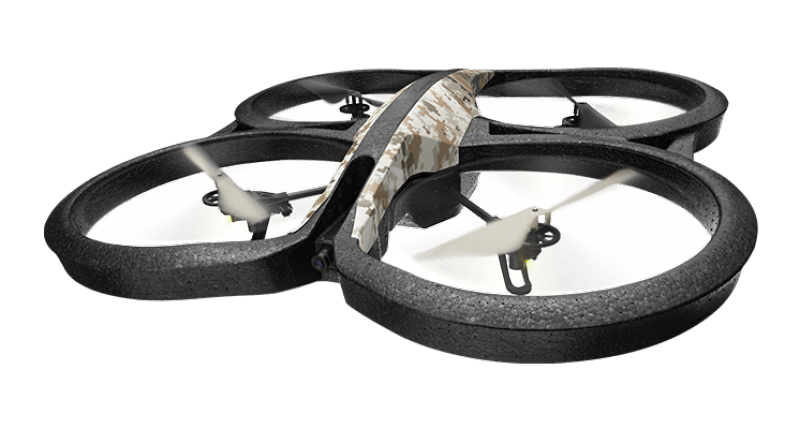
\includegraphics[scale=0.5]{Bilder/ar_drone.png}
	\caption{Parrot AR.DRONE 2.0 Elite Edition \cite{dronepicture}}
	\label{fig:ardrone}
\end{figure}

%https://www.parrot.com/fr/sites/default/files/styles/product_teaser_hightlight/public/parrot_ar_drone_gps_edition.png?itok=0shlzcXW
Diese zeichnet sich unter Anderem durch eine Frontkamera mit einer Auflösung von 1280×720 Pixeln und einer Bildrate von 30 fps aus. Weiterhin ist Sie mit einer zum Boden gerichteten QVGA Kamera ausgerüstet, welche 60 Bilder pro Sekunde aufnimmt. \newline
Die Drohne orientiert sich beim Fliegen mit Hilfe einer Vielzahl von Sensoren. Dazu gehören ein dreiachsiges Gyroskop und ein Magnetometer. Weiterhin nutzt sie Beschleunigungs-, Ultraschall- und Luftdrucksensoren. \newline
Der Grund für die Wahl der Drohne ist vor allem der vergleichsweise niedrige Preis von ca. 200€ und der starken Verbreitung in der Forschung. Dadurch gibt es bereits eine Vielzahl von Projekten, die dazu führen, dass die Drohne und das dazugehörige Interface zu einem großen Umfang fehlerfrei funktionieren. \newline
Weiterhin gibt es schon ROS Nodes (siehe \ref{ROS}) und konfigurierte Modelle in Simulationsumgebungen, welche die Arbeit an dem Projekt beschleunigen.


\section{ROS}
%Max
\label{ROS}
\subsection{Allgemeines}
%Max
Das Robotic Operating System, kurz ROS, ist eine Sammlung von Softwareframeworks für die Entwicklung von Software für persönliche Roboter. Es stellt entsprechende Bibliotheken und Werkzeuge zur Verfügung, um Entwicklern die Programmierung zu vereinfachen. Dabei bietet ROS einem Betriebssystem ähnliche Funktionalitäten auf Basis eines homogenen Computercluster. Dazu gehören Hardwareabstraktion, low-level Steuerung, Nachrichtevermittlung zwischen verschiedenen Prozessen und Paketmanagement. Trotz der Notwendigkeit hoher Reaktivität und geringer Latenz bei der Steuerung von Robotern handelt es sich es de facto nicht um ein richtiges Betriebssystem , obwohl es durch den Namen(\grqq Operating System\grqq) suggeriert wird. Dennoch ist es möglich Echtzeitcode (\grqq realtime code\grqq) in ROS zu integieren \cite{realtimecode}. ROS ist eins der am meisten genutzten Frameworks und hat eine stark wachsende Gemeinschaft, was es in Kombination mit dessen Features zu einer enorm wichtigen Technologie macht.\cite{rosbook} \cite{rosgeneral}


\subsection{Design Prinzipien}
Das Robotic Operating verfolgt fünf grundlegende Design Prinzipien: 
\begin{itemize}
	\item Peer-to-Peer
	\item werkzeugbasiert
	\item Mehrsprachigkeit
	\item Unabhänigkeit
	\item Open Source
\end{itemize}
\textbf{Peer-to-Peer:} Im Normalfall besteht ein Roboter aus mehreren Komponenten und oft aus verschiedenen Recheneinheiten. Oft gibt es einen zentralen leistungsstarken Rechner der unabhängig vom Roboter existiert, welcher für die Koordination und rechenintensive Aufgaben, wie zum Beispiel Bildverarbeitung verantwortlich ist. Da dieser oft wegen Mobilitätsgründen nicht per Kabel mit dem Roboter verbunden ist, geschieht die Kommunikation mittels WLAN oder vergleichbaren drahtlosen Kommunikationsmitteln. Dies kann unter Umständen sich schnell zu einem Flaschenhals entwickeln, da große Datenmengen transportiert werden müssen, wenn die zentrale Einheit für den Datentransport zuständig ist. Daher baut ROS auf ein Peer-to-Peer Konzept auf bei dem zentrale Einheit sich lediglich darum kümmert die kommunizierenden Nodes vor Kommunikationsbeginn miteinander verbindet. Dafür ist lediglich ein Auskunftsmechanismus notwendig, der Prozessen oder ähnlichem ermöglicht korrespondierende Kommunikationspartner zur Laufzeit zu finden und eine Verbindung herzustellen. Somit können mögliche Flaschenhälse entschärft werden.\cite{rosbook}\cite{rosconcepts}\newline 
\textbf{Werkzeugbasiert:} Dabei handelt es sich um ein weiteres grundlegendes Prinzip um die Benutzbarkeit zur vereinfachen und gleichzeitig eine höher Modularität zu gewähren. Anstelle eines großen komplexen Werkzeug zum Arbeiten mit ROS, existieren mehrere kleine Werkzeuge die dem Single-Responsibility-Prinzip(SRP)\cite{singleresp} folgen, also nur eine konkrete Aufgabe haben. Dieses Prinzip lässt sich mit eine Mikroservice-Architektur vergleichen, wobei es sich allerdings um Werkzeuge handelt und keine Services.
\newline
\textbf{Mehrsprachigkeit:} Damit möglichst viele Systeme an ROS angebunden werden können und auch die Vorteile einzelner Programmiersprachen ausgereizt werden können, existiert das Prinzip der Mehrsprachigkeit. Somit wird es dem Nutzer ermöglicht die Sprache mit der programmieren will, frei zu wählen und erhöht den Nutzkomfort. Momentan werden C++, Python und Lisp durch sogenannte ROS Client Libraries. Weiterhin existieren experimentelle Client Libaries für Sprachen GO, Haskell, Java und viele weitere.\cite{clientlibary}
\newline
\textbf{Unabhängigkeit:} Die Kopplung der Software mit der Hardware bei Robotikszenarien ist immer relativ hoch, da die Treiber meistens plattformspezifisch sind. Um allerdings die Wiederverwendbarkeit diverser Algorithmen zu fördern, setzt man darauf die Algorithmen möglichst unabhängig vom jeweiligen Roboter zu implementieren, sodass sie im Optimalfall bei jedem System Anwendung finden können. Entwickler stellen die entsprechenden als Bibliotheken zur Verfügung und die starke Kopplung wird etwas entschärft.\cite{rosbook}\cite{rosconcepts}
\newline
\textbf{Open Source:} Da ROS unter der BSD-Lizenz\footnote{siehe: http://www.linfo.org/bsdlicense.html} steht, kann es sowohl für nicht-kommerzielle Projekte als auch kommerzielle Projekt verwendet werden. Der Source Code ist öffentlich zugänglich. Entwickler können ihre eignen Module beliebig lizenzieren.\cite{rosbook}\cite{rosconcepts}


\subsection{ROS Nodes}
%Max
ROS baut auf einem einfachen Konzept auf, dem Publish-Subscribe Pattern, bei welchem ein Publisher ein Nachricht mit einem festem Thema verschicken kann und ein beliebiger Subscriber, der sich für das Thema interessiert, ist in der Lage diese zu empfangen, zu verarbeiten und unter Umständen erneut zu versenden.  Somit besteht eine ROS Anwendung aus der Regel aus vielen kleinen Teilen, den sogenannte Nodes. Jede Node hat ihre eigenen Aufgabe und kann auf diverse Themen registrieren, sogenannte Topics. Für diese Topics werden von anderen Nodes Nachrichten publiziert, welche empfangen und verarbeitet werden können. Ist die Verarbeitung abgeschlossen, besteht die Möglichkeit die verarbeiteten Daten für andere Nodes zur Verfügung zu stellen, in dem sie mit einer neuen Topic publiziert werden. Somit kann eine Node sowohl Publisher, als auch Subscriber sein. 
Topics werden in ROS durch einen festen Nachrichtentyp definiert. Dessen exakter Aufbau muss vor Verwendung deklariert werden um einen einheitlichen Nachrichtenaustausch zu gewähren. Wie in der Abbildung unterhalb zu sehen, wird der Nachrichtentransfer durch eine zentrale Einheit geregelt, sodass Daten wirklich nur die Nodes erreichen, die sich auch dafür registriert haben. Dieser zentrale Bestandteil ist in ROS der Roscore, bei welchem sich alle Nodes zur Erstellung registrieren. Sozusagen eine Masternode, welche sich um die Verwaltung der anderen Nodes kümmert. Im Unterschied zum Pattern kümmert sich der Core nur um die anfängliche Vermittlung der Nodes untereinander. Er stellt somit sicher, dass sich die Nodes untereinander finden können. Er fungiert in diesem Falle als ein sogenannter Message Broker\cite{messagebroker}, was eine Erweiterung des klassischen Eventbus-Muster ist\cite{eventbus}. Weiterhin können ROS Nodes Services anbieten. Im Gegensatz zum regulären Nachrichtenaustausch basiert ein Serviceaufruf auf dem Request Response Prinzip, das heißt wenn ein Service aufgerufen wird, erhält der Aufrufer definitiv eine Antwort. Hierbei wird der Aufruf auch nicht über eine Topic realisiert, sondern die Node wird konkret angesprochen und muss dafür aktiv sein.\cite{rosbook}\cite{rosconcepts}
\begin{figure}[ht]
		\centering
	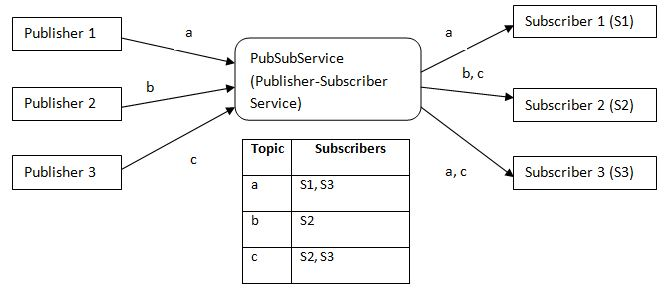
\includegraphics[scale=0.7]{Bilder/pubsub1.jpg}
	\caption[Publish-Subscribe Pattern]{Publish-Subscribe Pattern}

\end{figure}
\newline
ROS Nodes können in verschiedenen Sprachen implementiert werden, da die Kommunikation über die festen Nachrichtentypen geschieht, welche über den Roscore ausgetauscht werden. Dadurch ist es möglich Nodes in C++, Python und ebenfalls Lisp zu programmieren. Wodurch das ganze Konzept enorm flexibel gestaltet wird. Die fest definierten Nachrichtentypen verhindern, dass es an den Schnittstellen zu Problemen kommt und Nachrichten von allen Nodes einheitlich empfangen und versendet werden. \newline
Durch diese Modularität ist einfacher Komponenten und Funktionalitäten sowohl zu verwalten, als auch zu warten. Ebenfalls sind durch einheitliche Schnittstellen der Austausch von Nodes einfach und ermöglicht ein flexibles Ökosystem.

%%%%%%%%%%%%%%%%%%%%%%%%%%%%%%%%
%TODO: siehe Kommentar
% Wie wäre es, wenn wir noch sowas wie \subsection{Software Qualität} oder so machen
% und dann noch catkin build (vll auch im vergleich zu dem standard rosbuild) beschreiben
% dazu vll noch das wir alles mit startup scripten und so automatisiert haben, keine ahnung
% wäre noch ein guter filler und könnte man mit erwähnen - wäre hier in deinem Teil mit drin

%%%%%%%%%%%%%%%%%%%%%%%%%%%%%%%%
%\subsection{Software Qualität}
%Um die Qualität der Anwendung zu sichern wird Catkin Build anstelle des %veralteten rosbuild verwendet. Bei Catkin sind Pakete der atomare Bestandteil der Anwendung.
%TODO%http://wiki.ros.org/catkin_or_rosbuild 

\section{Simulation mit Gazebo}
Da es besonders beim Flug von Quadrocoptern schnell zu Schäden kommen kann und das sowohl  in langen Ausfallzeiten resultieren kann, als auch zu erhöhten Materialkosten führt ist es sinnvoll Testflüge in simulierte Umgebungen auszulagern. Speziell beim Test von autonomen Verhalten ist der Test der Features in realer Umgebung somit mit hohem Risiko verbunden. Um dies zu vermeiden ist die Simulation von Quadrocoptern und verschiedener Umgebungen unabdingbar. Ebenfalls erleichtert eine simulierte Version der Drohne die Entwicklung, da sie nicht immer physikalisch vorhanden sein muss. Dabei ist es allerdings notwendig, insbesondere
bei Bilddaten, dass die reale Situation möglichst realitätsnah abgebildet wird, sodass
das Verhalten im realen Umfeld entsprechend ähnlich ist. Insbesondere bei der
Verarbeitung von Kameradaten ist es allerdings abzuwägen ob Ergebnisse in der Simulation
mit Resultaten in realen Umgebungen vergleichbar sind, da die simulierten
Bilddaten in der Regel eher steril sind.\newline
Durch die Integration von ROS kommt die Simulationsumgebung Gazebo als Bestandteil
mit. Anfänglich handelte es sich um ein ROS Paket, mittlerweile ist es allerdings
ein eigenständiges Ubuntupaket und benötigt de facto kein ROS zur Laufzeit.
\newline
Da die realistische Simulation einer Drohne sehr umfangreich ist wird das ROS Paket "tum simulator" verwendet. Es enthält eine Implementation der AR Drone 2.0 für den Gazebo Simulator. Es wurde von Hongrong Huang und Jürgen Sturm
 aus der Computer Vision Group von der Technischen Universität München entwickelt.\cite{tumsim} Die Drohne wird komplett abstrahiert, wodurch die Simulation sich ohne Veränderung mit der realen Drohne austauschen lässt. 
 \begin{figure}[ht]
 	\centering
 	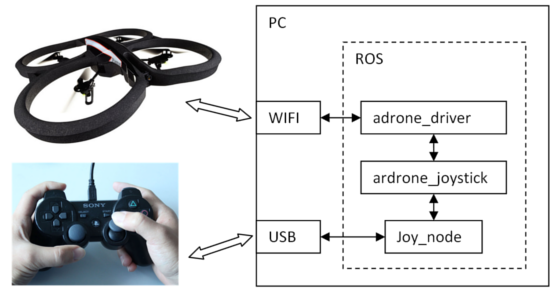
\includegraphics[scale=0.9]{Bilder/real_structure.png}
 	\caption[Programmstruktur mit dem realen Quadrocopter]{Programmstruktur mit dem realen Quadrocopter \cite{real_structure}}
 	
 \end{figure}
 Es ist auch möglich sowohl den Quadrocopter real zu steuern, als auch gleichzeitig in der Simulation. Das ermöglicht einen direkten Vergleich zwischen simulierten und realen Ergebnisse, vorausgesetzt, dass die simulierte Umgebung der echten annähernd entspricht.
  \begin{figure}[ht]
  	\centering
  	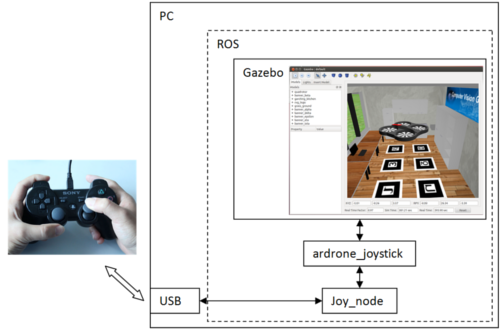
\includegraphics[scale=1.0]{Bilder/sim_structure.png}
  	\caption[Programmstruktur unter Verwendung von Gazebo]{Programmstruktur unter Verwendung von Gazebo \cite{sim_structure}}
  	
  \end{figure} %Max
Die Steuerung der Drohne, wird bei dem Package nativ über einen Playstation 3 Controller realisiert. Dessen Eingaben werden von der ROS-Node "Joy Node" verarbeitet und anschließend an die Node "ardrone joystick" weitergeleitet. Dort werden die Daten entsprechend übersetzt um entweder von Gazebo und/oder der realen Drohne verwendet werden zu können. Wenn sie an den realen Quadrocopter gesendet werden sollen, müssen sie noch entsprechend vom "ardrone driver" übersetzt werden, da lediglich Bitfolgen per WLAN versendet werden. 
\section{Fuzzylogik}
\subsection{Allgemeines}
Fuzzylogik, englisch fuzzy für unscharf oder verschwommen, ist eine Theorie die 1965 von Lotti Zadeh entwickelt wurde. Sie beschäftigt sich mit dem Modellierung von unscharfen Wissen und wird hauptsächlich für die Kontrolltheorie,sowie künstliche Intelligenz verwendet. Im Gegensatz zur klassischen Logik, die als Ergebnis nur wahr oder falsch zulässt, kann man mit Fuzzylogik auch die Ausprägung einer Zugehörigkeit feststellen. Diese sogenannte \textit{Fuzziness} ermöglicht Zuordnungen wie \grqq stark\grqq \space oder \grqq ziemlich\grqq. Wesentliche Elemente sind linguistische Variablen, welche, was der Name impliziert, Wörter und Ausdrücke anstellen von Zahlen verwenden um diese unscharfen Mengen zu repräsentieren. Diesen wird eine Funktion zugeordnet um die jeweilige Ausprägung der Variable feststellen zu können.\cite{fuzzylogik} \newline
Im folgenden werden fachspezifische Terme aus der Fuzzylogik verwendet, dafür werden nachfolgende Grundbegriffe kurz erklärt:
\begin{itemize}
	\item Unscharfe Menge (fuzzy set): Mathematisches Konzept zur Darstellung vager Angaben, welches teilweise Mengenzugehörigkeit erlaubt.\cite{fuzzybook}\cite{WissensbasierteSysteme}
	\item Unscharfe Logik (fuzzy logic): Isomorphes Konzept zur Unscharfen Menge, welches sich um den Umgang mit graduell ausgeprägten Wahrheitswerten kümmert.\cite{fuzzybook}\cite{WissensbasierteSysteme}
	\item Unscharfe Regel (fuzzy rule): Simple Regel, deren Prädikate unscharfe Mengen enthält.\cite{fuzzybook}\cite{WissensbasierteSysteme}
	\item Unscharfes Schließen (fuzzy reasoning): Formalisierung und Auswertung der unscharfen Regelbasen durch einen mathematischen Rahmen.\cite{fuzzybook}\cite{WissensbasierteSysteme}
	\item Unscharfe Regelung (fuzzy control): Einbindung unscharfer regelbasierter System in technischen Anwendungen, wird auch als Fuzzy Interferenz bezeichnet \cite{fuzzybook}\cite{WissensbasierteSysteme}. 
\end{itemize}
Das verwendete Fuzzymodell besteht insgesamt aus acht linguistischen Variablen, vier Ein- und Ausgabevariablen, von welchen jede fünf Zugehörigkeitsfunktionen besitzt. Weiterhin gibt es einen Regelblock um aus den Eingaben auf die entsprechenden Ausgaben zu schließen.

\subsection{Fuzzylite}
Für die Implementation der Fuzzylogik wird die C++ Bibliothek FuzzyLite von Juan Rada-Vilela verwendet. Es handelt sich dabei um eine gratis Opensource Libary und unterstützt alle gängigen Funktionen der Fuzzylogik.\cite{fuzzylite}  
\begin{lstlisting}[caption=Beispielcode zur Erzeugung eines neuen Fuzzymodells]
void FuzzyController::init() {
	engine = new Engine;
	engine->setName("input");
	InputVariable* backward = new InputVariable;
	backward->setName("backward");
	backward->setEnabled(true);
	backward->setRange(-1.000, 1.000);
	backward->addTerm(
	new Trapezoid("strongForward", -1.000, -1.000, -0.800, -0.400));
	backward->addTerm(
	new Trapezoid("mediumForward", -0.900, -0.600, -0.400, 0.000));
	backward->addTerm(
	new Trapezoid("mediumBackward", 0.000, 0.400, 0.600, 0.900));
	backward->addTerm(
	new Trapezoid("strongBackward", 0.400, 0.800, 1.000, 1.000));
	engine->addInputVariable(backward);
}
\end{lstlisting}
Mit dem Code erzeugt man zunächst eine neue Engine und anschließend eine Eingabevariable. Dieser wird ein Wertebereich zugewiesen und Zugehörigkeitsfunktionen erstellt. Schlussendlich wird die Variable bei der Engine registriert. 
\begin{lstlisting}[caption=Code zur Erzeugung von einem Regelsystem]
RuleBlock* ruleBlock = new RuleBlock;
ruleBlock->setEnabled(true);
ruleBlock->setConjunction(new Minimum);
ruleBlock->setDisjunction(new Maximum);
ruleBlock->setImplication(new Minimum);
ruleBlock->setActivation(new General);
ruleBlock->addRule(Rule::parse(
"if backward is strongForward then backwardSpeed is strongForward",
engine));
engine->addRuleBlock(ruleBlock);
\end{lstlisting}
Mit diesem Code erzeugt man ein neues Regelsystem und fügt eine beispielhafte Regel hinzu. Ein komplettes System besteht aus wesentlich mehr Regeln, da es normalerweise komplex ist.
\begin{lstlisting}[caption=Code zur Auswertung des Regelsystems]
backward->setValue(back);
sideward->setValue(side);
up->setValue(upValue);
rotation->setValue(rotateRight);
engine->process();
\end{lstlisting}
Schließlich kann man den Eingabevariablen konkrete Werte zuweisen und das System mithilfe von unscharfen Schließen auswerten.

\section{Kinect}
%Max
\subsection{Allgemeines}
Um Gesten des Benutzers zur erkennen und entsprechend auszuwerten wird der visuelle Sensor Microsoft Kinect verwendet. Normalerweise wird er zur Steuerung der Videospiel Konsole Xbox360/Xbox One verwendet. Das System ist in der Lage Tiefenbilder zu erstellen, besitzt sowohl eine 1080p Farbkamera, als auch einen Infrarotsensor und mithilfe mehrere Mikrofone Sprache und Bewegung im Raum zu erkennen. Anhand der verschiedenen Kameraeingaben ist es möglich den Körper von bis zu 2 Nutzern zu erkennen und auch entsprechend zu verfolgen. Für Windows stellt Microsoft ein entsprechendes Software Development Kit (SDK) zur Verfügung um die Benutzung der Funktionalität zu vereinfachen.\cite{kinectgolem} \cite{kinectms} \cite{kinectSDK}
\subsection{Vergleich der verschieden Stacks zur Implementation}
Für ROS existieren zwei Stacks für die Verwendung des Kinect Sensors:
\begin{itemize}
	\item Freenect Stack\cite{freenect}
	\item OpenNI Stack\cite{openni}
\end{itemize}
Beide Implementationen liefern einen Treiber um den Sensor anzusprechen und die Kameradaten auszulesen. Allerdings gibt es auch einige Unterschieden zwischen den zwei Stacks. Der Freenect-Treiber ermöglicht es neben den Kameradaten ebenfalls die LED, einen Beschleunigungssensor, sowie die Audiodaten der Kinect zu bedienen.\cite{freenect} Dies ist mit dem Treiber von OpenNI allerdings nicht möglich. Dafür kommt auf dessen Stack noch ein Tracker mit dem es möglich ist Benutzer zu erkennen und deren Bewegungen zu tracken. Ebenfalls ermöglicht OpenNI die Segmentation der Bilddaten, Handerkennung und Gestensteuerung. Die extrahierten Merkmalspunkte können weiter verwendet werden. Beide Implementierungen sind Open Source und stehen unter der Apache2.0 Lizenz\cite{opennilicense}\cite{freenect}. Durch das Skeletontracking biete OpenNI allerdings einiges an Vorteilen für die Implementation der Steuerung, daher fällt die Wahl auf diesen Stack, da für die Usecase wesentlich besser passt.
%Max

\section{Punktwolken}
\label{Punktwolken}
%Christoph
Die Tiefenbilder die REMODE erstellt sind in Form von sogenannten Punktwolken, bzw. Point Clouds. Diese Punktwolken sind eine Menge von Punkten in einem Vektorraum, welche jeweils durch ihre Raumkoordinaten in einem dreidimensionalen kartesischen Koordinatensystem beschrieben sind. Somit ist jedes Element im Datensatz durch die Attribute $X$, $Y$ und $Z$ gekennzeichnet. \cite{defPC}\cite{visPC}\ \newline
Sobald ein Tiefenbild approximiert wurde, werden diese Informationen über das ROS Topic \textit{/remode/depth/pointcloud} geteilt. \newline

\begin{figure}[ht]
	\centering
	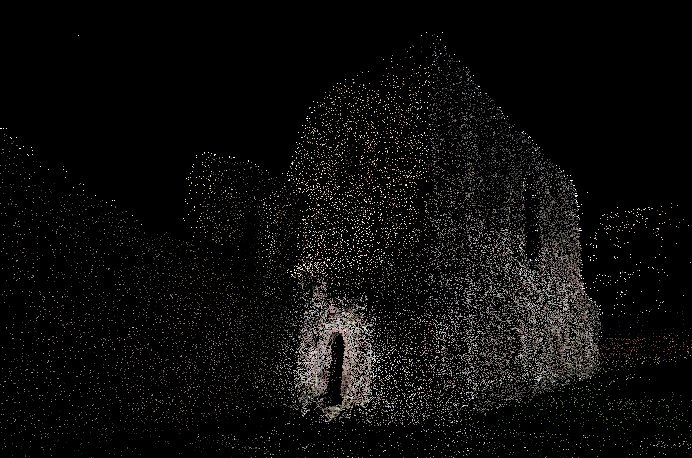
\includegraphics[scale=0.41]{Bilder/pointcloud_1.jpg}
	\label{fig:pointcloud}
	\caption{Beispiel einer visualisierten Punktwolke \cite{visPC}}
\end{figure}

Die Darstellung zeigt beispielhaft die Visualisierung einer Punktwolke. Dabei entscheidet die Helligkeit der Punkte über ihre relative Tiefe in Bezug zur Kamera. Der Vektorraum $V \in \mathbb{R}^3$ mit den entsprechenden Datenpunkten wird das ROS Topic in einem Intervall von wenigen Sekunden übertragen.\newline

\section{Point Cloud Library}
%Christoph

Die Punktwolken, wie in Abschnitt \ref{Punktwolken} beschrieben, bilden die Grundlage, um essentielle Auswertungen und Analysen für das Assistenzsystem auszuführen. Da hierfür teilweise komplexe Algorithmen und mathematische Berechnungen notwendig sind, würde die eigene Implementierung den Rahmen dieser Arbeit sprengen. \newline
Das OpenSource Projekt Point Cloud Library \emph{PCL} stellt für diesen Anwendungsfall in dessen Programmbibliothek zahlreiche Algorithmen bereit, die einfach implementiert werden können. Diese helfen bei Problemen der 2D und 3D Bildverarbeitung, sowie der Punktwolkenverarbeitung. %cite http://pointclouds.org/
Dabei werden Anwendungen in der Bildverarbeitung bereitgestellt, wie die Filterung, Segmentierung und Visualisierung von Punktwolken. \newline
Zusätzlich verfügt die PCL eine Schnittstelle zu ROS, wodurch sie sich bestens in die Projektumgebung integrieren lässt.
%\chapter{Weit hinter den Wortbergen}
\label{cha:wortberge}





Weit hinten, hinter den Wortbergen, fern der Länder Vokalien und Konsonantien leben die Blindtexte. Abgeschieden wohnen Sie in Buchstabhausen an der Küste des Semantik, eines grossen Sprachozeans. Ein kleines Bächlein namens Duden fliesst durch ihren Ort und versorgt sie mit den nötigen Regelialien.

Es ist ein paradiesmatisches Land, in dem einem gebratene Satzteile in den Mund fliegen. Nicht einmal von der allmächtigen Interpunktion werden die Blindtexte beherrscht - ein geradezu unorthographisches Leben.

Eines Tages aber beschloss eine kleine Zeile Blindtext, ihr Name war Lorem Ipsum, hinaus zu gehen in die weite Grammatik. Der grosse Oxmox riet ihr davon ab, da es dort wimmele von bösen Kommata, wilden Fragezeichen und hinterhältigen Semikoli, doch das Blindtextchen liess sich nicht beirren. Es packte seine sieben Versalien, schob sich sein Initial in den Gürtel und machte sich auf den Weg.

Als es die ersten Hügel des Kursivgebirges erklommen hatte, warf es einen letzten Blick zurück auf die Skyline seiner Heimatstadt Buchstabhausen, die Headline von Alphabetdorf und die Subline seiner eigenen Strasse, der Zeilengasse. Wehmütig lief ihm eine rethorische Frage über die Wange, dann setzte es seinen Weg fort.

Unterwegs traf es eine Copy. Die Copy warnte das Blindtextchen, da, wo sie herkäme wäre sie zigmal umgeschrieben worden und alles, was von ihrem Ursprung noch übrig wäre, sei das Wort "und" und das Blindtextchen solle umkehren und wieder in sein eigenes, sicheres Land zurückkehren.

Doch alles Gutzureden konnte es nicht überzeugen und so dauerte es nicht lange, bis ihm ein paar heimtückische Werbetexter auflauerten, es mit Longe und Parole betrunken machten und es dann in ihre Agentur schleppten, wo sie es für ihre Projekte wieder und wieder missbrauchten.

Und wenn es nicht umgeschrieben wurde, dann benutzen Sie es immer noch.


\textbf{}
%\begin{figure}[htb]
%\centering
%\includegraphics[width=0.8\textwidth]{FHWTLogo.jpg}
%\caption{Das Logo der FHWT}
%\label{fig:FHWTLogo}
%\end{figure}



\chapter{Software Architektur}
\section{Anforderungen}
\label{sec:Anforderungen} 
%Christoph

Im Folgenden sollen die Anforderungen an die Studienarbeit festgelegt werden. Diese gliedern sich in viel Hauptbestandteile auf. \newline
Der erste Teil besteht darin, ein bestehendes Vorgängerprojekt in eine andere Umgebung zu portieren. Das Projekt ermöglicht die Steuerung einer AR.Drone 2.0 mit Hilfe von Gesten. Die Gesten sind vorgeschriebene Positionen der Arme. So soll der Nutzer beispielsweise mit einer Bewegung von beiden ausgestreckten Armen, nach oben und unten, die Drohne starten, steigen, senken und landen lassen können. \newline
Dabei wurde die Erkennung der Positionen mit einer Kinect Stereo Kamera von Microsoft umgesetzt. Die Daten der Kamera werden im Programmcode verarbeitet. Dieser wurde in der Sprache \textit{C\#} geschrieben und funktioniert auf Grund einer Vielzahl von externen Libraries, wie die Anbindung der Kinect, nur unter Windows. \newline
Als Grundlage für die weiteren Ziele dieser Arbeit soll dieses Projekt für UNIX basierte Betriebssysteme umgeschrieben werden. Grundlage für die Softwarearchitektur bildet das ROS Framework, welches eine Modularisierung der Projektbestandteile in ROS Nodes vorgibt. Ziel soll es sein, die Funktionalität des Bestandsprojektes vollständig nachzubilden. \newline
Die zweite Anforderungsteil besteht darin, dass jegliche Funktionalität auch in einer Simulation verfügbar sein soll. Somit kann man für Präsentationen, in denen der Flug einer Drohne nicht möglich ist, den Quadrocopter in einer frei gestaltbaren, simulierten Umgebung fliegen lassen. \newline
Es soll in diesem Zusammenhang möglich sein, problemlos zwischen einer realen und einer simulierten Drohne wechseln zu können.
Ein weiterer Bestandteil dieser Arbeit umfasst die Approximation von Tiefeninformationen. Dafür soll ausschließlich eine unveränderte AR.Drone verwendet werden, welche nur mit einer monokularen\footnote{Monokular ist die Bezeichnung für Kameras mit einer einzelnen Linse} Frontkamera ausgestattet ist. \newline
Um aus den Bildern dieser Kamera Tiefenbilder zu gewinnen, soll ein externes Projekt in die Projektlandschaft integriert werden. Hierbei soll es wiederum möglich sein, dass der Videostream sowohl von der realen, als auch von der simulierten Drohne gesendet werden kann. Es soll dabei ermittelt werden, ob die Nutzung der externen Arbeiten für den Anwendungszweck praktikabel und sinnvoll ist. \newline
Der vierte Bestandteil dieser Arbeit besteht im Erarbeiten, Testen und Bewerten von möglichen Ansätzen und Limitationen der Implementierung eines Assistenzsystems. Das Ziel ist es herauszufinden, wie mit den Tiefeninformationen die manuelle Steuerung der Drohne durch eine Person, mit Hilfe von Assistenzfunktionen, unterstützen werden kann. \newline
Ein Anwendungsbeispiel ist hierbei das sichere Fliegen durch ein Hindernis wie eine offene Tür, oder das verhindern von Kollisionen mit Objekten in der Umgebung.
\newpage
\section{Bildverarbeitung}
\label{Bildverarbeitung}
In diesem Abschnitt wird beschrieben, wie die Position der Kamera im Raum bestimmt werden kann, um anschließend aus aufeinanderfolgenden Aufnahmen Tiefeninformationen zu gewinnen. Die beschriebenen Implementierungen beziehen sich dabei auf die Arbeit von Christian Forster, Matia Pizzoli und Davide Scaramuzza, welche ihre Abhandlungen zum Thema zusammen mit dem Programmcode frei zugänglich gemacht haben.

\subsection{Semi-Direct Monocular Visual Odometry - SVO}
%Christoph
Eine Grundanforderung an das Projekt ist die Nutzung einer nicht modifizierten AR.Drone. Dadurch entsteht die Problematik, dass keine Tiefenbildkamera genutzt werden kann, um in Echtzeit Tiefenbilder zu erhalten. Die Drohne ist lediglich mit einer monokularen Frontkamera ausgestattet. \newline
Um Tiefeninformationen aus den Bildern einer solchen Kamera zu gewinnen, wird eine Szene aus verschiedenen Perspektiven aufgenommen. Anschließend gibt es unterschiedliche Ansätze um aus den aufeinanderfolgenden Bildern Kamerapositionen und Umgebungsstrukturen zu ermitteln. \newline
Feature basierte Ansätze sind der aktuelle Standard zur Berechnung der Kamerapostion. Diese versuchen die wichtigsten Merkmale eines Bildes, die Features, zu extrahieren. Mit Hilfe von Feature Deskriptor Algorithmen werden Vektoren mit Informationen zu invarianten Bildbereichen berechnet. Diese Vektoren verhalten sich wie ein einzigartiger Fingerabdruck, der die Merkmale repräsentiert. \newline
Aufeinanderfolgende Bilder werden dann mit Hilfe dieser Deskriptoren abgeglichen und sowohl Kamerabewegungen, als auch Strukturen werden rekonstruiert. Zur Optimierung sind abschließend die ermittelten Kamerapositionen anzugleichen. Dies geschieht mit Hilfe von Algorithmen zur Minimierung des Reprojektionsfehlers.\footnote{Reprojektionsfehler sind geometrische Fehler die im Zusammenhang zwischen abgebildeten und berechneten Bildpunkten entstehen. \cite{repro}} 
\newline
Ein weiterer Ansatz ist die direkte Methode. Hierbei werden die Features nicht über Deskriptor Algorithmen bestimmt, sondern das Problem wird über die Intensitäten der Pixel gelöst. Bei einem Graustufenbild entspricht diese Intensität der Helligkeit von Bildbereichen. \newline
Somit kann bei der Rekonstruktion im Gegensatz zum Feature basierten Ansatz auch die Richtung der Gradienten von Intensitäten genutzt werden. Dadurch funktioniert diese Methode auch bei Bildern mit sehr wenig Textur, Bewegungsunschärfe und fehlerhaftem Kamerafokus. \newline
Das für diese Arbeit relevante Vorgehen kombiniert die Vorteile der beschriebenen Methoden. Die semi-direkte Odometrie\footnote{Odometrie bezeichnet die Verwendung Bewegungssensordaten zur Bestimmung der Positionsänderung über die Zeit.\cite{hodor}} verwendet einen Algorithmus der ebenfalls auf Zusammenhängen von Features basiert. Diese werden jedoch implizit aus einer direkten Bewegungsabschätzung bezogen, anstatt explizit durch Algorithmen mit Feature Deskriptoren berechnet zu werden. \newline
Dadurch müssen Features nur extrahiert werden, wenn diese noch nicht auf einem der vorherigen Bildern vorhanden waren. \newline
Insgesamt ist dieser Ansatz sehr schnell, da wenig Berechnungen pro Bild stattfinden und auf Grund der Verwendung von Intensitätsgradienten äußerst genau und robust. \newline
Diese Eigenschaften sind für die Anforderungen der Studienarbeit essentiell, da die Drohne sich sehr schnell bewegen kann und somit in möglichst kurzer Zeit neue Bilder auswerten muss. Das beschrieben Verfahren minimiert damit die Auswirkungen der typischen Probleme von Drohnen. Diese sind einerseits die niedrige Texturierung der Umgebung, welche hauptsächlich in Innenräumen auftritt und andererseits kameraspezifische Probleme wie Bewegungsunschärfe und der Verlust des Kamerafokus. \newline
Im Folgenden zeigt die Abbildung wie die Nutzung von SVO in der Praxis aussieht.
\begin{figure}[ht]
	\centering
	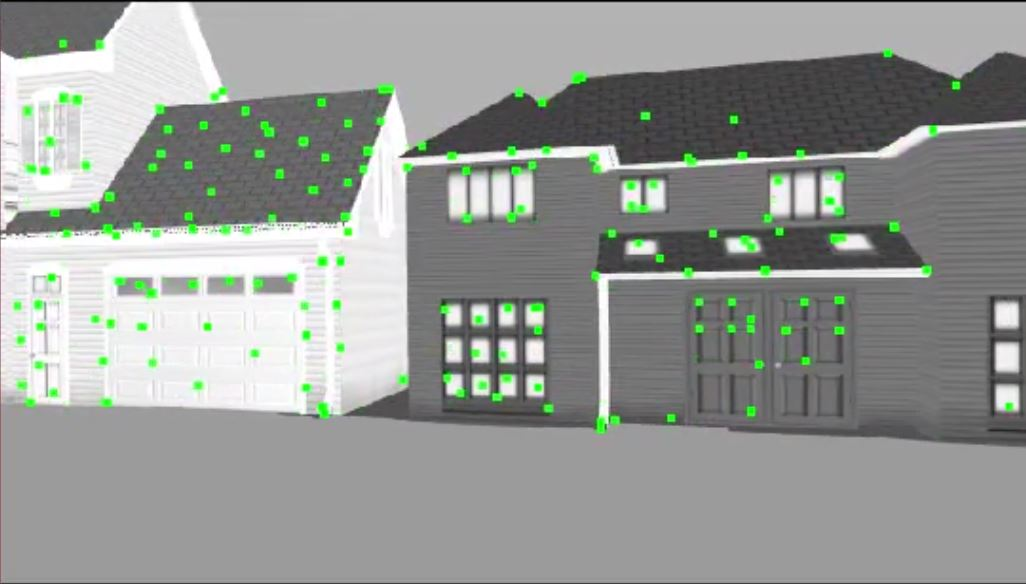
\includegraphics[scale=0.7]{Bilder/SVO.jpg}
	\label{fig:svo}
	\caption{Semi-Direct Monocular Visual Odometry im Simulator}
\end{figure}

Hierbei stammt das Kamerabild von einer Drohne im Simulator Gazebo in einer frei verfügbaren Testwelt mit einigen Gebäuden. Die grünen Punkte sind die Features, die SVO anhand der beschriebenen Strategie ermittelt hat. \newline
Die Anzahl der aktuell gefundenen Features kann dabei stark variieren. Diese Schwankung entsteht hauptsächlich durch die unterschiedliche Texturierung und Anzahl der Kanten von Objekte in der Umgebung. \newline
Weiterhin kann auch die Kamera selbst ein Grund für eine geringe Anzahl gefundener Features sein. Gründe und Lösungen dafür werden im Folgenden beschrieben.

\subsection{Kamerakalibrierung}
%Christoph
Ein Grundproblem der Bildverarbeitung ist die Verzerrung des Bildes. 
Da die Bestimmung der Kameraposition möglichst genau sein soll, muss die Kamera vorher kalibriert werden. Dies bedeutet, dass Ungenauigkeiten der Linse erkannt und softwareseitig ausgeglichen werden. Dafür werden die intrinsischen Parameter der Kamera bestimmt \newline

\subsubsection*{Kalibrierungsmodelle}
Hierbei unterstützt SVO drei Kamera Modelle: ATAN, Ocam und Lochkamera. \cite{svo_cameracalibration} \newline
Das ATAN Modell basiert auf dem \textit{Field of View \emph{(FOV)}} Verzerrungsmodell "Straight lines have to be straight [...]" von Devernay und Faugeras.\newline %cite https://hal.inria.fr/inria-00267247/document
Der Vorteil dieser Kalibrierungsmethode ist die äußerst schnelle Berechnung der Projektion des Bildes. % cite https://github.com/uzh-rpg/rpg_svo/wiki/Camera-Calibration
Das Modell vernachlässigt jedoch tangentiale Verzeichnung, welche auftritt, wenn optische und mechanische Bestandteile des Objektives, sowie der CCD-Sensor 
\footnote{CCD steht für \emph{charge-coupled device}, was übersetzt ladungsgekoppeltes Bauteil bedeutet. Dieses lichtempfindliche elektronische Bauteil wird zur Bildaufnahme verwendet.} 
nicht perfekt zueinander ausgerichtet sind. % cite http://www.aishack.in/tutorials/major-physical-defects-cameras/
Weiterhin sollte die Kamera mit einem globalem Shutter ausgestattet sein, um die Extraktion von Bildmerkmalen bei Bewegungen zu gewährleisten. Kameras mit Global-Shutter-CMOS  
\footnote{CMOS steht für \emph{Complementary metal-oxide-semiconductor} und ist ein spezieller Halbleiter der zur Bildaufnahme verwendet wird.} % cite https://de.wikipedia.org/wiki/Complementary_metal-oxide-semiconductor
Sensoren und CCD-Sensoren nehmen Bild nicht zeilen- und spaltenweise, sondern vollständig auf und sind daher für das Verfahren geeignet. \newline
Die Drohne besitzt eine veraltete und günstige Kamera mit einem CMOS Sensor, wodurch sowohl tangentiale Verzerrung, als auch der Rolling-Shutter-Effekt auftreten können. \newline
%cite https://dspace.cvut.cz/bitstream/handle/10467/66885/F3-DP-2017-Pahorecky-Petr-priloha-ARDrone_Developer_Guide.pdf?sequence=-1&isAllowed=y
Daher ist das ATAN Modell zwar eine der besten Kalibrierungsmethoden für teure Hochleistungskameras, jedoch ist es für die Betrachtungen dieser Arbeit nicht optimal. \newline
Der zweite Ansatz zur Kalibrierung ist das Ocam Modell von Davide Scaramuzza. Diese Methode sollte für Kameras mit sehr weitem Sichtfeld, oder omnidirektionalen Kameras genutzt werden. Damit ist es für die Drohne nicht geeignet. \newline
Die dritte unterstützte Kalibrierungsmethode ist das Modell der \textit{Lochkamera}, bzw. auf Englisch \textit{Pinhole Model}.
Der Name und das zugrunde liegende Prinzip basieren, wie der Name es sagt, auf der Lochkamera. Die Abbildung zeigt die grundsätzliche Funktionsweise. \newline
\begin{figure}[ht]
	\centering
	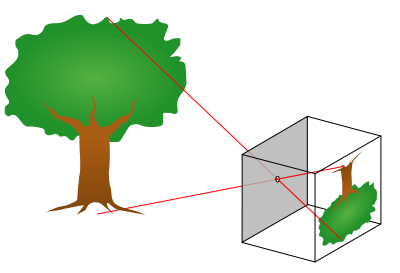
\includegraphics[scale=0.5]{Bilder/pinhole.png}
	\label{fig:pinhole}
	\caption{Prinzip der Lochkamera \cite{lochkamera}}
\end{figure}

Die Darstellung zeigt, dass bei der Lochkamera Licht durch eine kleine Öffnung in einen kleinen Hohlkörper fällt. Dadurch entsteht auf der Rückseite ein auf dem Kopf stehendes Bild. \newline
Bei dem Pinhole Model handelt es sich um den aktuellen Standard in OpenCV \footnote{``OpenCV is the leading open source library for computer vision, image processing and machine learning, and now features GPU acceleration for real-time operation.''} %cite https://developer.nvidia.com/opencv
und ROS. Hierbei wird die Verzerrung mit Hilfe von fünf intrinsischen Parametern beschrieben, welche im Rahmen der Kalibrierung bestimmt werden müssen.

\begin{figure}[ht]
	\centering
	
\includegraphics[scale=0.7]{Bilder/distortion.png}
	\label{fig:distortion}
\end{figure}

OpenCV betrachtet dabei radiale und tangentiale Faktoren. Die Formel für radiale Verzeichnung ist die Folgende:

\begin{figure}[ht]
	\centering
	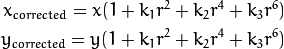
\includegraphics[scale=0.7]{Bilder/radialFactors.png}
	\label{fig:radial}
\end{figure}

Hierbei wird aus einem alten Bildpunkt $(x,y)$ des Eingabebildes die korrigierte Position $x_{corrected} y_{corrected}$ bestimmt. \newline
Die Berechnung der tangentialen Verzerrung erfolgt durch die Formel:

\begin{figure}[ht]
	\centering
	
\includegraphics[scale=0.7]{Bilder/tangentialFactors.png}
	\label{fig:radial}
\end{figure}

Abschließend werden die Einheiten angepasst:

\begin{figure}[ht]
	\centering
	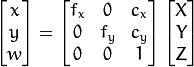
\includegraphics[scale=0.7]{Bilder/matrixEquation.png}
	\label{fig:radial}
\end{figure}

Dabei entspricht $f_x$ und $f_y$ der Brennweite der Linse und $c_x$, sowie $c_y$ beschreiben die optische Bildmitte in Pixelkoordinaten. \newline
% cite http://docs.opencv.org/2.4/doc/tutorials/calib3d/camera_calibration/camera_calibration.html
Dieser Ansatz ist der einfachste und funktioniert grundsätzlich mit jeder Kamera.

\subsubsection*{Umsetzung der Kalibrierung}
Um die intrinsischen Parameter der Kamera zu bestimmen, wird ein bekanntes Bild oder Muster aufgenommen. Dazu wird ein Vergleich zwischen den theoretischen und tatsächlichen Abmessungen angestellt. Hierzu wird meist ein einfaches Schachbrettmuster genutzt, welches im möglichst vielen verschiedenen Perspektiven aufgenommen wird. Bei der realen Drohne wird dazu das Muster ausgedruckt, bei der Simulation muss hingegen ein muss ein solches Objekt in die Welt eingefügt werden. Da die Kamera in der Simulation ohnehin keine intrinsischen Fehler aufweisen sollte, kann auf eine Kalibrierung verzichtet werden. \newline

\begin{figure}[ht]
	\centering
	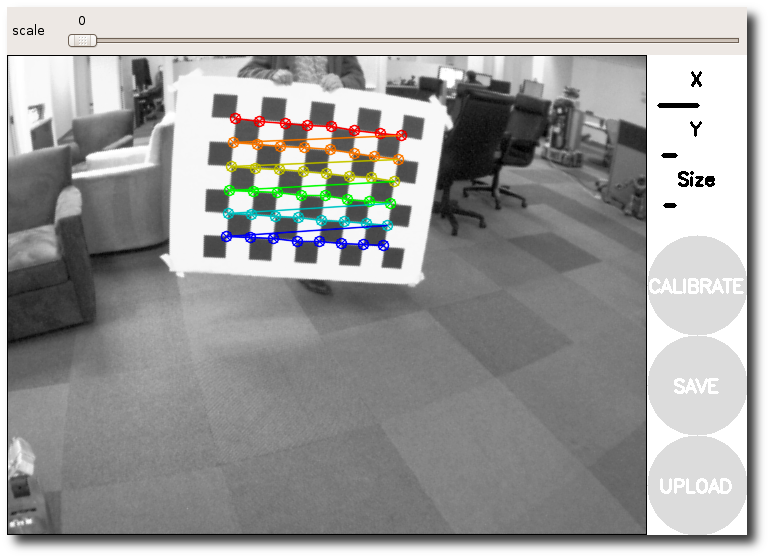
\includegraphics[scale=0.4]{Bilder/calibrationChecker.png}
	\label{fig:calibrationChecker}
\end{figure}

Die Kalibrierung wurde mit dem frei verfügbaren ROS Node \textit{camera\_calibration} umgesetzt. Das Ergebnis ist abhängig von der Anzahl der Perspektiven und der Qualität der Aufnahmen. Aufgegeben wird dann die List der Parameter, die für das Lochkamera Modell notwendig sind.

\subsection{Regularized Monocular Depth Estimation - REMODE}
%Christoph
Im vorherigen Abschnitt wurde beschrieben, wie anhand von aufeinanderfolgenden Bildern die Position der Kamera im Raum bestimmt werden kann. Dieses Problem wird seit mehr als 20 Jahren untersucht und wird als Structure From Motion \emph{SFM} in der Bildverarbeitung und Simultaneous Localization and Mapping \emph{SLAM} in der Robotik bezeichnet. \newline
%Smith, R.C.; Cheeseman, P. (1986). "On the Representation and Estimation of Spatial Uncertainty" (PDF). The International Journal of Robotics Research. 5 (4): 56–68. 
Um den Nutzer aktiv bei der Steuerung der Drohne zu unterstützen werden jedoch Tiefeninformationen benötigt. Dazu müssen Tiefenbilder und Tiefenkarten (footnote) aus den Bildern der monokularen Kamera bestimmt werden. \newline
Für diesen Schritt gibt es unterschiedliche Ansätze. Der State of the Art ist die Berechnung mit Hilfe des Bayes-Schätzers. Dabei handelt es sich um eine Schätzfunktion in der mathematischen Statistik, welche eventuell vorhandenes Vorwissen bei der Schätzung eines Parameters berücksichtigt. Dabei wird in der bayesschen Statistik das initiale Vorwissen mit Hilfe der A-priori-Verteilung modelliert, die bedingte Wahrscheinlichkeit des Parameters unter Betrachtung dieses Vorwissens mit der A-posteriori-Verteilung. \newline
%http://www.mathematik.uni-ulm.de/stochastik/lehre/ss04/statistik1/skript/node26.html
Im Umfang dieser Arbeit wird die Forschung und Implementierung des Projekts Regularized Monocular Depth Estimation \emph{REMODE} genutzt. In dieser Ausarbeitung von Matia Pizzoli, Christian Forster und Davide Scaramuzza wird die bayessche Schätzung mit neusten Entwicklungen in der Konvexoptimierung verbunden. Hierbei stützen sie ihre Forschungen auf die Ergebnisse von G. Vogiatzis und C. Hernandez und ihrer Abhandlung mit dem Titel ''Video-based, real-time multi-view stereo`` von 2011. \newline
REMODE erfüllt den Zweck, mit Hilfe der gewonnenen Informationen ein dreidimensionales Modell des Raumes zu erstellen. Die Abbildung zeigt ein Beispiel dazu, welches von den Entwicklern verbreitet wurde. \newline

\begin{figure}[ht]
	\centering
	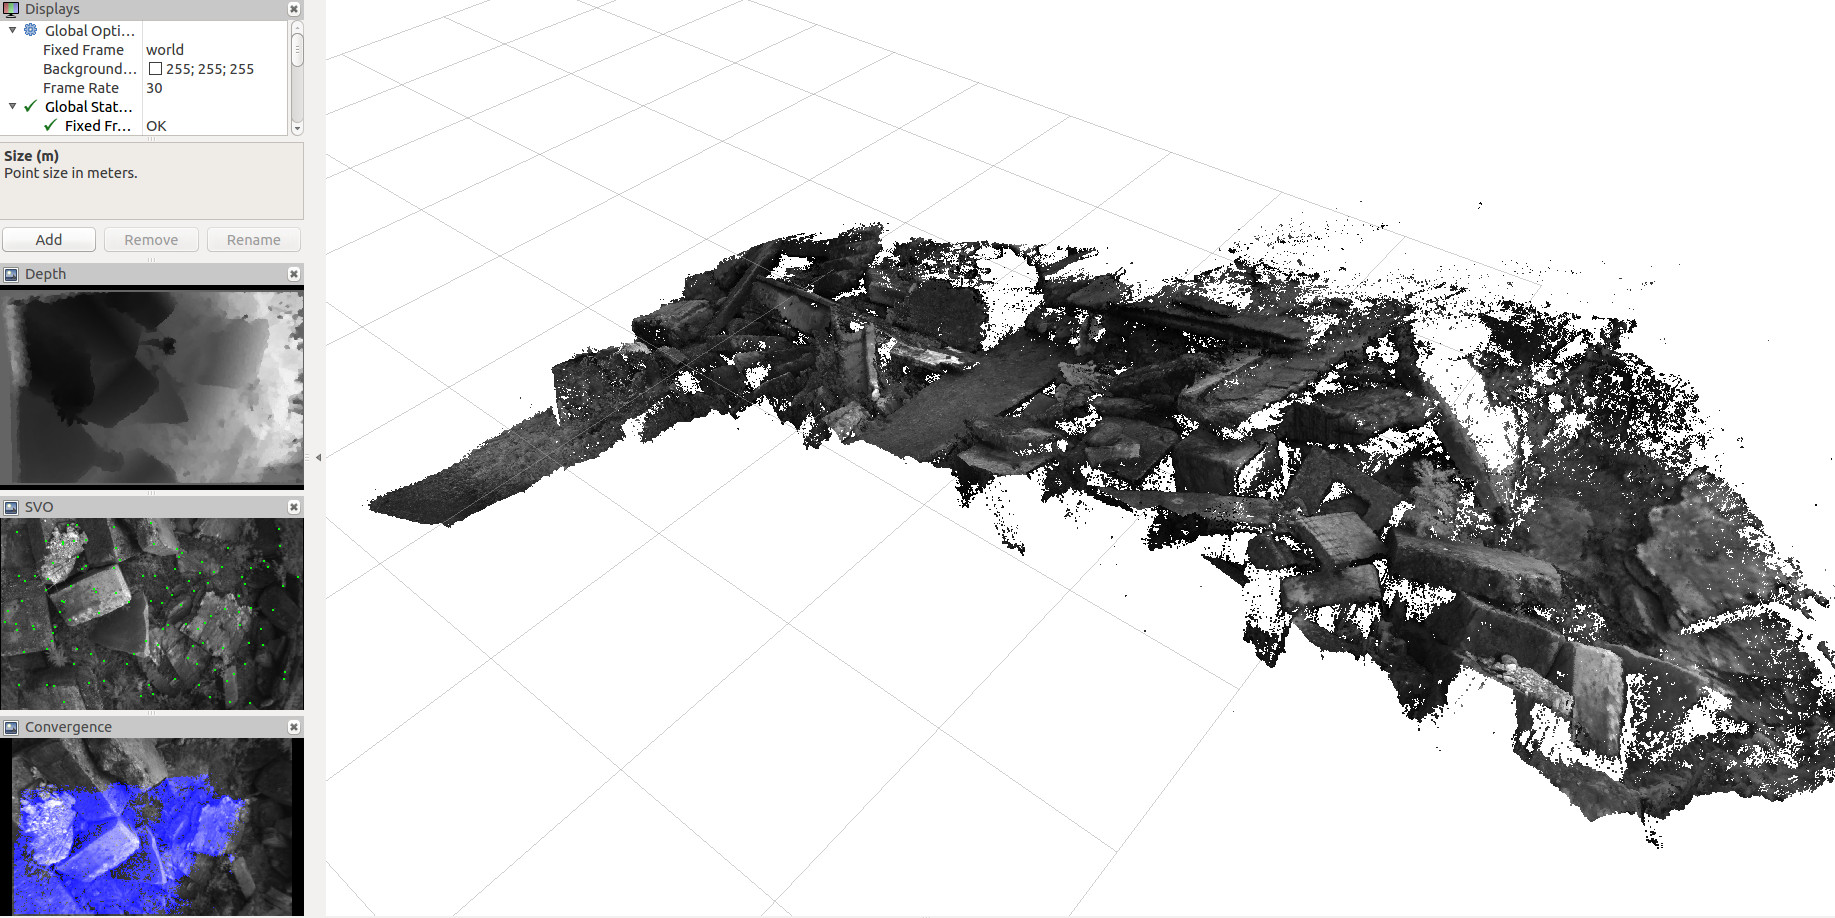
\includegraphics[scale=0.22]{Bilder/remode_3dmodel.jpg}
	\label{fig:pinhole}
	\caption{REMODE 3D-Modell, Flug über Trümmer \cite{remode3d}}
\end{figure}

Die Darstellung zeigt ein 3D Modell eines Trümmerhaufens, welches mit Hilfe der aufeinanderfolgenden Einzelbildern generiert wurde. Die Visualisierung erfolgte mit dem Standard 3D Visualisierungstool für ROS, genannt \textit{RVIZ}. \newline
REMODE ermöglicht eine Berechnung der Tiefeninformationen in Echtzeit und auf Pixelbasis. Weiterhin ist die aktuelle Genauigkeit und Fehlerrate im Vergleich zur Realität zu jeder Zeit sichtbar. \newline
Im Folgenden wird der grundsätzliche Ansatz der Implementierung skizziert. Die genauen Details übersteigen dabei auf Grund der hohen Komplexität den Umfang dieser Arbeit.

\begin{figure}[ht]
	\centering
	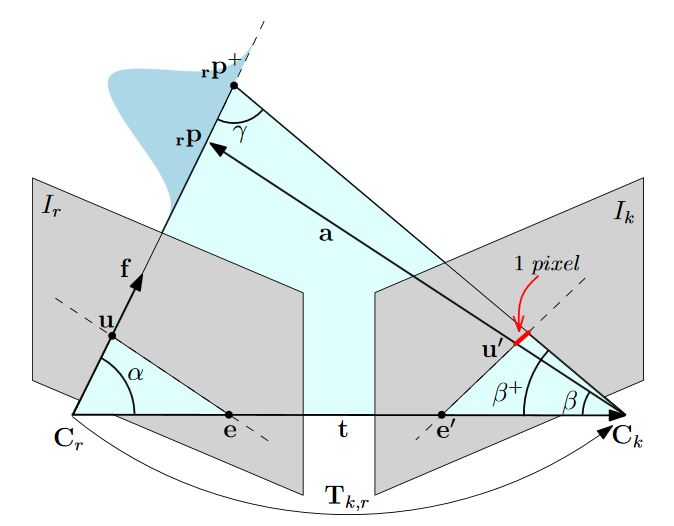
\includegraphics[scale=0.7]{Bilder/REMODE_overview.jpg}
	\label{fig:radial}
\end{figure}

In der Übersicht sieht man die beiden Kamerapositionen $I_r$ und $I_k$ mit den zugehörigen Kamerazentren $C_r$ und $C_k$. Die Positionen im Raum dieser Kameras wurden im vorherigen Schritt mit Hilfe von SVO ermittelt. $T_k,r$ zeigt dabei die starre Transformation der Kamerabilder. \newline
Der Punkt $r_P$ ist die aktuelle Schätzung der Position eines Punktes auf den epipolaren Flächen.
Die Varianz der Abweichung von einem Pixel auf der epipolaren Linie durch estrich und ustrich wird berechnet mit der Gleichung tkquadr.
Mit Hilfe der oben angesprochenen mathematischen und statistischen Auswertungen kann nun die Tiefe eines Punktes $r_P$ approximiert werden. \newline
Das Zusammenspiel von SVO und REMODE ist für handelsüblichen Laptops mit CPU und GPU ausgelegt. Dabei läuft SVO komplett auf dem Prozessor und REMODE verwendet das Framework NVIDIA CUDA, (footnote) was auf den Grafikchip des Rechners zugreift. \newline
Die Implementation setzt auf eine durchschnittliche Bewegung der Kamera von 0.0038 Meter pro Sekunde und einer mittleren Tiefe von einem Meter bei einer Berechnungszeit von 3.3 ms pro Bild. \newline



\subsection{Performanceprobleme}
\label{performanceprobleme}
%hier mal vollkommen auslassen über alle performanceissues

Trotz der Nutzung neuster Methoden und Techniken zur Berechnung der Kamerapositionen und Tiefenbilder, gibt es Probleme hinsichtlich der Performance. Dabei ist das Hauptproblem die Differenz im verfolgten Ziel zwischen dieser Arbeit und der Implementierung von SVO und REMODE. \newline
Der Hauptanwendungszweck ist ein langsamer, stetiger Flug einer Drohne über ein Gebiet. Dabei zeigt die aufnehmende Kamera nach unten und hat sowohl eine sehr hohe Qualität, als auch ein großes Sichtfeld von mehr als 110 Grad. Die Bewegungen der Drohne sind nur nach seitlich, nach vorne und nach hinten, nicht jedoch um die eigene Achse. Somit wird sicher gestellt, dass immer genügend Referenzfeatures vorhanden sind, damit zu jedem Zeitpunkt die Position der Kamera bekannt ist. \newline
Im Gegensatz dazu sind die Anforderungen der Arbeit stark abweichend. So ist sowohl die Qualität, als auch die Verarbeitung der Kamera minderwertig. Auch das Blickfeld ist mit 90 Grad deutlich zu klein, wodurch weniger Features auf einem Bild Platz finden. \newline
Dadurch, dass die Kamera nach vorne und nicht nach unten gerichtet ist, treten weitere Komplikationen auf. Gleiche Bewegungen verursachen somit größere Änderungen am Bild, wodurch mehr Berechnungen notwendig werden und somit die Fehleranfälligkeit steigt. Vor allem Drehbewegungen um die eigene Achse sorgen für erhebliche Änderungen und führen meist zum Abbruch von SVO. \newline
Auch die Kalibrierung der Kamera der realen Drohne war auf Grund der schlechten Qualität schwierig. So konnte der Richtwert des Reprojektionsfehlers von rund 0,1 Pixel nicht erreicht werden, sondern lag eher bei 0,3 Pixel. \newline
Bei Tests in Innenräumen mit der AR.Drone konnte SVO nicht mehr als 50 Features finden. Um jedoch die Position der Kamera zu bestimmten, sind mehr als 100 Features notwendig.
Diese Beobachtungen aus den Testläufen decken sich mit den Hinweisen zur Performance in der Projektdokumentation\cite{svodocs}. \newline


\newpage
\section{Implementierung}
\subsection{Grundlegende Herausforderungen}
Es bestand eine nicht modularisierte, schlecht dokumentierte C\# Dokumentation für eine Windowsumgebung. Diese galt es teilweise für ROS zu übernehmen. Für Windows existiert ein Kinect Software Development Kit, welches die Programmierung erleichtert.


\newpage
\subsection{Kinect}
Der visuelle Sensor Microsoft Kinect dient als Nutzerschnittstelle zur Bedienung, indem der Nutzer Gesten benutzt um die Drohne zu steuern. Um die Sensoreingaben richtig verwenden zu können sind 3 Schritte notwendig:
\begin{itemize}
	\item Korrekte Ansteuerung der Sensorhardware
	\item Körpererkennung und Tracking
	\item Verarbeitung der separaten Merkmale
\end{itemize}
Hierfür ist der erste Schritt die Hardware des Sensors richtig anzusteuern. Da die Microsoft Software nicht für Linux Systeme kompatibel ist, kommt einen Open Source Treiber zum Einsatz. Hierbei handelt es sich um OpenNI, welches auch eine Middleware bereit stellt um Körperbewegung und Gesten zur erkennen, sowie zu tracken. Die ROS-Node \grqq openni\_launch\grqq realisiert die Ansteuerung dess Kinect Sensors. Ebenfalls wird der zweite Schritt: Körpererkennung und Tracking  durch OpenNi gelöst, da die Middelware auch wie oben erwähnt dies kann. Das geschieht mithilfe der ROS-Node \grqq openni\_tracker \grqq. Für die den dritten Punkt: Verarbeitung der seperaten Merkmale ist die selbst implementierte ROS-Node "kinect\_controller" zuständig. Dort werden die durch OpenNI extrahierten Merkmale, wie zum Beispiel linke Hand, rechte Hand, Kopf, usw. als Grundlage eingegeben und Ziel ist es die entsprechenden Befehle anhand der Eingaben für den Quadrocopter zu erstellen.
%Max
\newpage
\subsection{Fuzzy Controller}
\subsection{Drone Controller}
\subsection{ROS Nodes}
Für den Gesamten Prozess von Nutzereingabe durch den Kinectsensor bis zur Steuerung der Drone werden eine Vielzahl von Komponenten benötigt, da einige Arbeitsschritte notwendig sind um die Daten zu verarbeiten. Zunächst wird die Microsoft Kinect durch die ROS-Node \grqq openni\_launch\grqq angesteuert und die Bilder der verschiedenen Kameras eingelesen. Anschließend werden diese Bilder durch die Node \grqq openni\_tracker \grqq analysiert und es wird, sofern ein Nutzer erkannt wurde ein Motion-Tracking erstellt. Dadurch werden bestimmte Features, in diesem Fall konkrete Körperteile erkannt. Diese werden als Nachricht unter der Topic \grqq/tf\grqq \space publiziert. Der kinect\_controller ist auf die Topic registriert und empfängt die gesendeten Nachrichten. Anhand der Merkmalspunkte werden vier Werte berechnet, die als Eingabe an die Fuzzy Logik übergeben werden. Anhand des Fuzzy Controllers ergeben sich vier Ausgangswerte, welche die Geschwindigkeiten für den Quadrocopter in den entsprechenden Richtungen,Neigung nach vorne/hinten, Neigung links/rechts, Rotation, sowie steigen/sinken angibt. Die Befehle werden an die Node 
\grqq drone\_controller\grqq übergeben wo sie nochmal verarbeitet werden. Dort ist der Ort wo auch das Assistenzsystem eingreifen kann, indem es Korrektureingaben an den Controller sendet und die Steuerbefehle des Nutzer anpasst oder gar verwirft. Schließlich wird der Befehl an den Treiber in der Node \grqq ardrone\_autonomy\grqq \space übergeben, auf Hardwareebene übersetzt und an den Quadrocopter oder die Simulation gesendet.
\begin{figure}[ht]
	\centering
	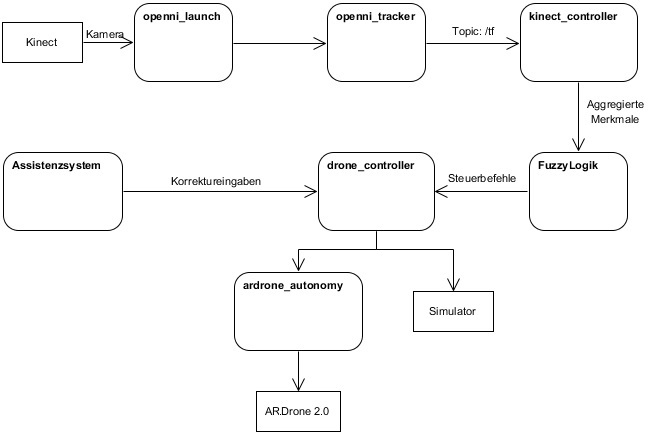
\includegraphics[scale=0.7]{Bilder/ros_nodes_flow.jpg}
	\label{Zusammenspiel der verschiedenen ROS-Nodes}
	\caption{Zusammenspiel der verschiedenen ROS-Nodes}
\end{figure}
%Beide
\newpage
\subsection{Architektur}
%Beide

\begin{figure}[ht]
	\centering
	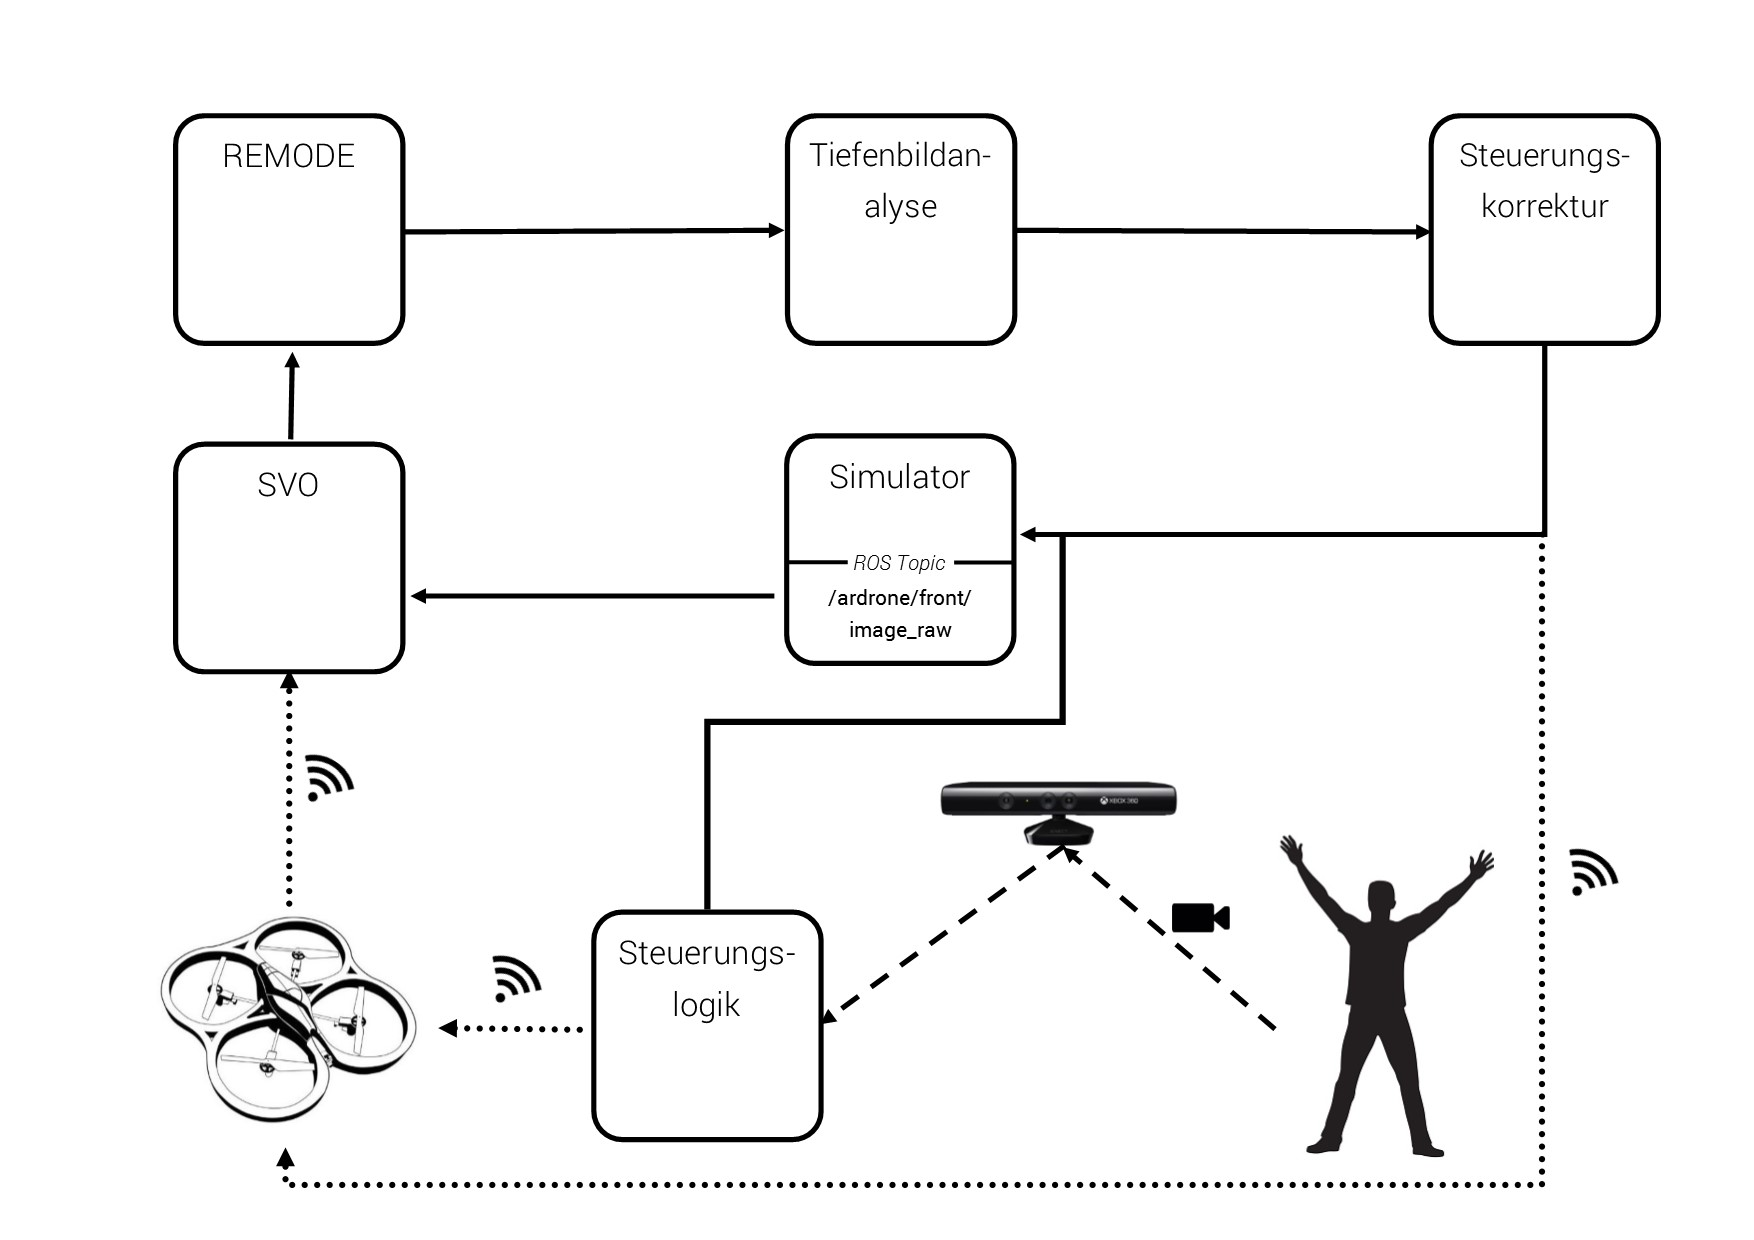
\includegraphics[scale=0.5]{Bilder/architecture.jpg}
	\label{fig:architecture}
	\caption{Übersicht zur Softwarearchitektur}
\end{figure}

%Bild der Drohne http://lightspots.ch/images/ARdronebw.png
%Bild vom Typ https://img.clipartfox.com/d02b01c31b79dd51b6c2c6a2a5db5985_stop-help-vector-art-outstretched-arm-clipart_416-416.jpeg
%Bild von kinect https://d3nevzfk7ii3be.cloudfront.net/igi/DtuTZhDHRWaOirBm.large


\newpage
\section{Assistenzsystem}
Im Kapitel \ref{Bildverarbeitung} wurde der Prozess beschrieben, wie aus den monokularen Aufnahmen der Frontkamera Tiefenbilder ermittelt werden können. Aufbauend darauf soll nun erarbeitet werden, wie mit Hilfe dieser Informationen die Implementation eines grundlegenden Assistenzsystems aussehen könnte.

\subsection{Problemanalyse}
%Christoph
Wie zuvor beschrieben, ist ein einfacher Anwendungsfall das Fliegen durch Hindernisse wie offene Türen. Dabei stößt man in der Bildverarbeitung auf eine Reihe von Herausforderungen. Wie in \ref{performanceprobleme} beschrieben, sind SVO und REMODE nicht optimal für den Anwendungsfall dieser Arbeit. Dabei treten Probleme vor allem bei der Analyse des Tiefenbildes auf. Dabei ist sowohl die niedrige Qualität der Tiefenbilder problematisch, als auch die hohe Zeit, welche zwischen den Bewegungen der Drohne und den Berechnungen der Tiefenpunktwolke vergehen kann. \newline
Die Folgende Darstellung zeigt ein Beispiel für ein von REMODE berechnetes Bild.

\begin{figure}[ht]
	\centering
	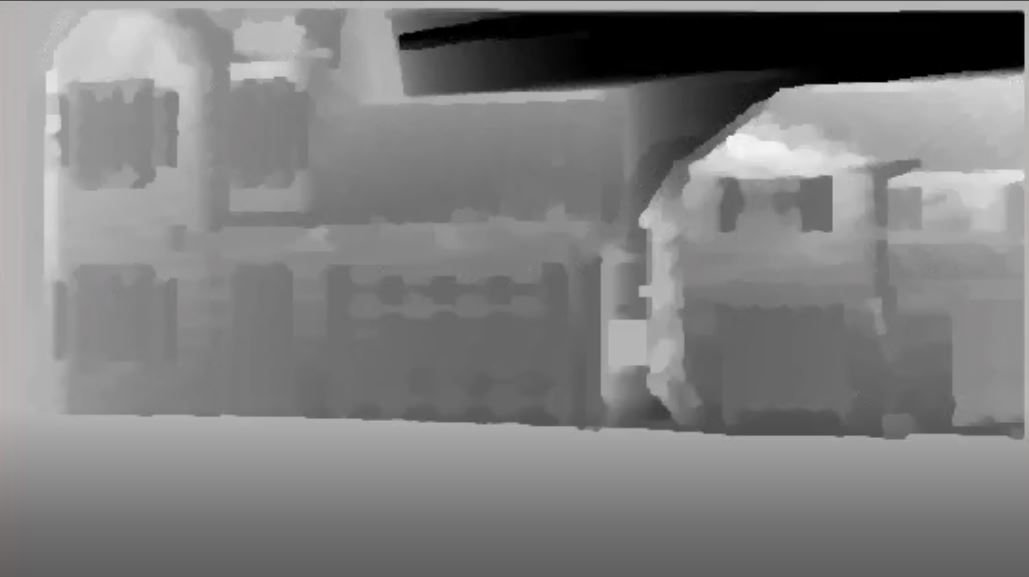
\includegraphics[scale=0.5]{Bilder/REMODE.jpg}
	\label{fig:REMODE}
	\caption{Approximiertes Tiefenbild durch REMODE}
\end{figure}

Dabei wird ersichtlich, das der grundlegende Kontext für einen menschlichen Betrachter verständlich ist - in diesem Fall sind dies zwei Häuser mit einer schmalen Lücke als Zwischenraum. Dabei sind genaue Texturen stark reduziert und teilweise verloren gegangen. Weiterhin sind Objektränder zum Teil von einem leichten hellen Schimmer umgeben, welcher in der Bildanalyse zu Problemen führen kann.


\subsection{Lösungsansätze}
Um an diesem Punkt ein Objekt wie eine Tür, bzw. den Zwischenraum zu erkennen, gibt es verschiedene Ansätze, um die Punktwolke zu analysieren.

\subsubsection{Referenzobjekt}
Eine Möglichkeit ist die gezielte Suche nach definierten Abmessungen, Abständen und Formen im Bild. Dabei wird das Zielobjekt in die einzelnen Teilabschnitte aufgeteilt und die relative Beziehung dieser Teilstücke beschrieben. Am Beispiel einer Tür entspricht dies dem Rahmen, welcher aus zwei, zueinander parallelen, Geraden besteht, die rechtwinklig auf dem Untergrund aufliegen. Die beiden Geraden werden am Ende durch eine rechtwinklige Gerade miteinander verbunden. \newline

\begin{figure}[ht]
	\centering
	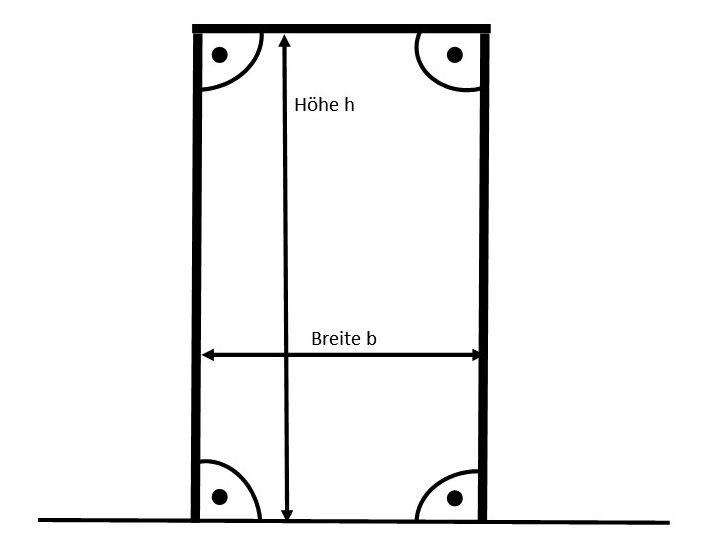
\includegraphics[scale=0.55]{Bilder/door.jpg}
	\label{fig:door}
	\caption{Objektreferenz einer Tür}
\end{figure}

Die Abbildung visualisiert die beschriebenen Anforderungen. \newline
Wie in der vorherigen Darstellung \ref{fig:REMODE} erkennbar, gibt es keine klaren Kanten und Abgrenzungen. Dies erschwert einen Vergleich mit dem Referenzobjekt zusätzlich. Abhilfe für dieses Problem schaffen in der Bildverarbeitung Filter. Filtern ist eine Technik um Bilddaten zu modifizieren, oder sie in einer Art zu verbessern. Hauptsächlich wird diese Methode dafür genutzt, um hohe Frequenzen in einem Bild zu verringern, also um das Bild zu glätten, oder um niedrige Frequenzen zu verstärken, also um Kanten hervorzuheben. \newline
Filter basieren auf einer Berechnung in der Nachbarschaft\footnote{Die Nachbarschaft um einen Pixel ist eine Menge an Pixeln, die sich durch ihre relative Distanz zu diesem auszeichnen. \cite{filter1}} von Pixeln, wobei der Wert eines gegebenen Pixels im Ausgabebild bestimmt wird, in dem Algorithmen auf Pixel in der direkten Nachbarschaft dieses Datenpunktes angewandt werden. \cite{filter1}   \newline
Da die Tiefenbilder verwaschen und unscharf sind, müssen niedrige Frequenzen verstärkt werden. Ein Standard, um Kanten in einem Bild hervorzuheben ist der Marr-Hildreth-Operator oder auch Laplacian of Gaussian \textit{LoG} genannt. \cite{LoG} Dieser Algorithmus führt auf den Matrizen der Punktwolken des Eingangsbildes Faltungsoperationen \footnote{todo; was ist faltungsoperation} durch, um ein Ausgabebild mit verdeutlichten Kanten zu erzeugen. \newline
Dabei sucht der LoG nicht nach Kanten, sondern nach Gebieten mit rapiden Änderungen von Pixelintensitäten. Die zweite Ableitung erzeugt eine Kurve, bei der die beiden Seiten einer Kante durch einen positiven und einen negativen Wert gekennzeichnet sind. Die eigentliche Kante liegt hierbei an dem Punkt, wo der Graph Null durchquert. Die Abbildung \ref{fig:LoG} verdeutlicht dieses Verhalten.
\begin{figure}[ht]
	\centering
	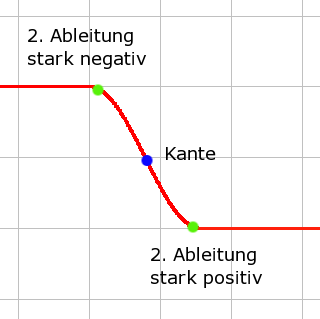
\includegraphics[scale=0.5]{Bilder/LoG.png}
	\label{fig:LoG}
	\caption{Verlauf der zweiten Ableitung im LoG Algorithmus \cite{LoG}}
\end{figure}
Die Point Cloud Library bietet dafür mit der Methode
\begin{center}
	\textit{pcl::Edge< PointInT, PointOutT >::detectEdgeLoG}
\end{center} 
eine Implementierung für diesen Algorithmus an. \cite{pclDocs} \newline
Nach dieser erste Schritt abgeschlossen ist, liegt ein Tiefenbild mit hervorgehobenen Kanten vor. Dies ist jedoch nicht ausreichend, um nun zuverlässig mit Hilfe eines Vergleichs mit dem Referenzobjekts z.B. Türen im Bild zu finden. \newline
Einerseits ist das Referenzobjekt grundsätzlich ein einfaches Rechteck. Diese gibt es potentiell sehr oft im Bild, wie beispielsweise Tische, Fenster oder Bilder an Wänden. Eine geöffnete Tür zeichnet sich dabei dadurch aus, dass der Inhalt des Rahmens weiter weg ist, also in der Punktwolke tiefer ist. Im Falle von sehr genauen Tiefenbildinformationen kann man an dieser Stelle mit einer hohen Wahrscheinlichkeit durch die Veränderung der Tiefe gute Ergebnisse bei der Suche erzielen. \newline
Wie bereits beschrieben ist das Tiefenbild jedoch sehr ungenau, da es nur durch einzelne Bilder approximiert wird. Somit ist die Verwendung eines Referenzobjektes und die Anwendung von Filtern zur Erkennung keine valide, praktisch einsetzbare Lösung. \newline

\subsubsection{Referenzpunktwolke}
Der zweite Ansatz basiert auf der Verwendung einer Referenzpunktwolke. Es wird somit kein relatives Objekt definiert, sondern man vergleicht die Punktwolke des gesamten Tiefenbildes, mit einer Punktwolke für eine Tür. \newline
Damit könnte ein besseres Ergebnis erzielt werden, da auch die Änderung der Tiefe zwischen Türrahmen und dem Bereich innerhalb des Rahmens betrachtet wird. Die Point Cloud Library bietet dafür eine Implementation an, welche als \textit{Correspondence Grouping}, also die Gruppierung nach Übereinstimmungen bezeichnet wird.

\begin{figure}[ht]
	\centering
	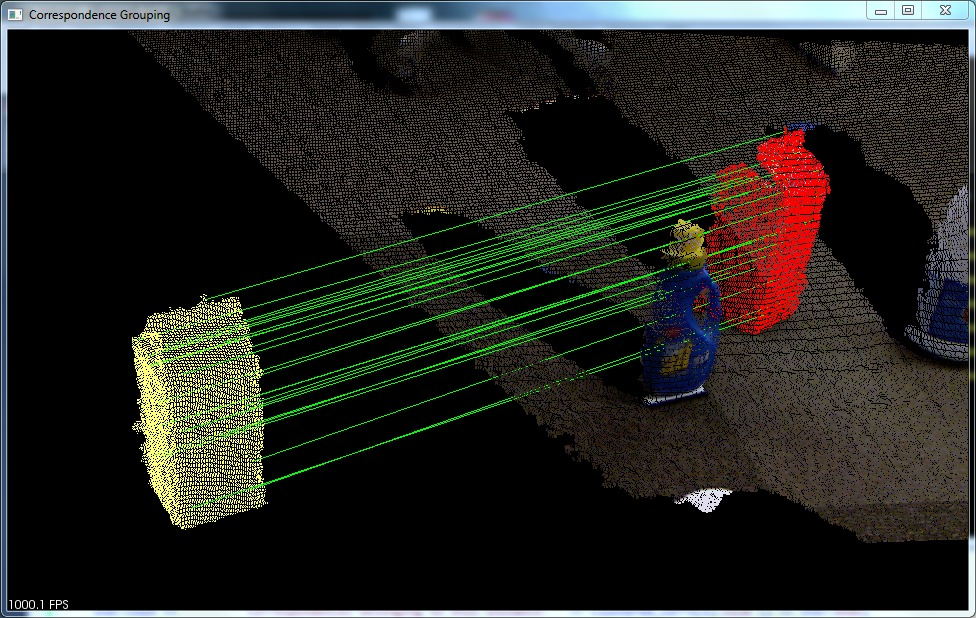
\includegraphics[scale=0.5]{Bilder/pcl_grouping.jpg}
	\label{fig:pcl_grouping}
	\caption{Correspondence Grouping mit dem PCL Algorithmus  \cite{pclGrouping}}
\end{figure}

Wie im Bild erkennbar wird mit Hilfe des Algorithmus versucht, Übereinstimmungen zwischen den Features der beiden Punktwolken zu finden. \newline
Schwierig ist hierbei die Auswahl und Generierung der Referenzpunktwolke. Es ist nicht möglich eine Lösung zu finden, die sowohl in der Simulation, als auch mit der realen Drohne funktioniert. Die Referenz ist immer nur dann sinnvoll, wenn sie nahezu exakt die gleichen Tiefeninformationen aufweist, wie das zu vergleichende Bild. \newline
Somit funktioniert die Auswertung auch nicht mehr, wenn eine leicht abgeänderte Tür verwendet wird, obwohl sich sowohl das Referenzobjekt, als auch das tatsächliche Objekt in der Simulation bzw. in der Realität befinden.
Weiterhin lassen sich die Tiefeninformationen eines bestimmten Objekts nur sehr schwer aus dem Gesamtbild extrahieren. Um dies zu erreichen müsste bereits bekannt sein, wo sich das Objekt im Bild befindet, also ein typisches Henne-Ei Problem. \newline
\subsubsection{Alternative Lösungen}
Weitere Überlegungen zur Objekterkennung sind spezielle Kennzeichnungen, die künstlich hinzugefügt werden. Denkbar sind beispielsweise farbliche Markierungen, wie ein roter Türrahmen, welcher sich farblich von der Umgebung abgrenzt und somit leicht zu finden ist. Dieser Ansatz ist grundsätzlich möglich und einfach umzusetzen, jedoch hat das Tiefenbild keine Farbinformationen. \newline
Es ist denkbar für dieses Zweck das Ausgangsbild zu verwenden, welches noch alle Farbinformationen besitzt, jedoch zweidimensional ist. Dies würde die Anforderungen an die Arbeit verletzen, da die Analyse nicht mehr auf den Tiefeninformationen basiert. \newline
Auch bei der Betrachtung anderer Objekte wie Wände kommt es zu schwerwiegenden Problemen. So kann der Abstand zwischen der Drohne und einer Wand in der Umgebung nicht genau genug bestimmt werden, um eine Kollision zu vermeiden, ohne unnötig in der Steuerung einzugreifen.
\chapter{Evaluation}
\section{Ergebnis}
%beide

%hier sollten wir vor allem die Probleme von SVO und REMODE ansprechen

\section{Ausblick}
%beide
%besserer simulator
%genaue Untersuchung mit PCL algorithmen
%svo und remode "umschreiben" bzw anpassen, sodass drehungen möglich sind etc

%\chapter{Summary}

\section{}

\section{}

\bibliography{references} 
\bibliographystyle{ieeetr}


% ---------------------------- Literaturverzeichnis ----------------------------------------------
% \begin{thebibliography}{999999}
% 
% \bibitem[1]{company} SAP offical website: \emph{SAP Company Information}, 2016.
% http://go.sap.com/corporate/en/company.html, \emph{visited: 08.22.2016}.
% \bibitem[2]{beacon1} Dejan Jurejevcic: \emph{IoT tech deep-dive: The rise of
% beacon technology}, 09.03.2015.
% https://iot-analytics.com/rise-of-beacon-technology/ \emph{visited: 08.22.2016}.
% \bibitem[3]{beacon2} Agnieszka Gasiorek: \emph{What Are Beacons & How Do They
% Work?}, 09.25.2014. https://kontakt.io/blog/infographic-beacons/, \emph{visited:
% 08.22.2016}.
% \bibitem[4]{usasmart} Monica Anderson: \emph{Technology Device Ownership: 2015},
% 10.29.2015.
% http://www.pewinternet.org/2015/10/29/technology-device-ownership-2015/,
% \emph{visited:
% 08.15.2016}.
% \bibitem[5]{iottech} Louis Columbus: \emph{Roundup Of Internet of Things
% Forecasts And Market Estimates, 2015}, 12.27.2015.
% http://www.forbes.com/sites/louiscolumbus/2015/12/27/roundup-of-internet-of-things-forecasts-and-market-estimates-2015/#739d8de148a0,
% \emph{visited:
% 08.23.2016}.
% \bibitem[6]{gsma} Sylwia Kechiche: \emph{Cellular M2M forecasts: unlocking
% growth}, 02.06.2015.
% https://www.gsmaintelligence.com/research/2015/02/cellular-m2m-forecasts-unlocking-growth/457/,
% \emph{visited:08.23.2016}.
% \bibitem[7]{sapranking} Truffle Capital: \emph{European software vendors ranking
% 2015}, 12.31.2015.
% http://www.truffle100.com/2015/ranking.php, \emph{visited:08.24.2016}. 
% \bibitem[8]{sapnewsm2m} SAP News: \emph{Ericsson and SAP Announce New
% Combination of Cloud-Based Machine-to-Machine Solutions to Enhance Enterprise
% Efficiency}, 02.25.2013.
% http://news.sap.com/ericsson-and-sap-announce-new-combination-of-cloud-based-machine-to-machine-solutions-to-enhance-enterprise-efficiency/,
% \emph{visited:08.17.2016}.
% \bibitem[9]{sapgocm} SAP Connected Manufacturing: \emph{Manufacturing Execution
% System (MES)}, unknown date.
% http://go.sap.com/product/enterprise-management/execution-mes.html,
% \emph{visited:08.16.2016}.
% \bibitem[10]{sapgoain} SAP Asset Intelligence Network: \emph{Seamlessly connect
% machines and business - with our asset intelligence repository}, unknown date.
% http://go.sap.com/germany/product/plm/asset-intelligence-network.product-capabilities.html,
% \emph{visited:08.16.2016}.
% \bibitem[11]{sapgolns} SAP Asset Intelligence Network: \emph{Seamlessly connect
% machines and business - with our asset intelligence repository}, unknown date.
% http://go.sap.com/solution/lob/supply-chain/logistics-network.html,
% \emph{visited:08.16.2016}.
% \bibitem[12]{hanaacid} Jim Gray: \emph{The Transaction Concept:
% Virtues and Limitations}, 06.1981.
% http://research.microsoft.com/en-us/um/people/gray/papers/theTransactionConcept.pdf,
% \emph{visited:08.17.2016}.
% \bibitem[13]{hana2} Franz Faerber, Sand Kyun Cha, Juergen Primsch, Christof
% Bornhoevd, Stefan Sigg, Wolfgang Lehner: \emph{SAP HANA Database - Data
% Management for Modern Business Applications}, 12.04.2011.
% ACM SIGMOD Record Volume 40 Issue 4, ACM New York, pp. 45-51.
% \bibitem[14]{sapiotstrats} Holger Mueller: \emph{First Take - SAP's IoT Strategy
% becomes clearer\ldots}, 01.28.2015.
% http://enswmu.blogspot.de/2015/01/first-take-saps-iot-strategy-becomes.html,
% \emph{visited:08.18.2016}.
% \bibitem[15]{hcpoff} SAP HANA Cloud Platform: \emph{What is SAP HANA Cloud
% Platform?}, unknown date.
% https://hcp.sap.com/index.html, \emph{visited:08.18.2016}.
% \bibitem[16]{hcpdocs} Developer Guide: \emph{SAP HANA Cloud Platform},
% 07.29.2016.
% https://help.hana.ondemand.com/help/frameset.htm, \emph{visited: 08.18.2016}.
% \bibitem[17]{sapvi} SAP Vehicle Insights: \emph{SAP Vehicle Insights: Create new
% business models with connected car analytics}, unknown date.
% http://go.sap.com/product/analytics/vehicle-insights.html,
% \emph{visited:08.18.2016}.
% \bibitem[18]{vidocs} Benjamin Graf, Ralf Ehret: \emph{Architecture Concept SAP
% Vehicle Insights}, 05.20.2015. Internal product documentation.
% \bibitem[19]{websocket1} Michael Carter: \emph{[whatwg] TCPConnection feedback},
% 06.2008.
% https://lists.w3.org/Archives/Public/public-whatwg-archive/2008Jun/0165.html,
% \emph{visited:08.18.2016}.
% \bibitem[20]{websocketbook} Andrew Lombardi: \emph{WebSocket: Lightweight
% Client-Server }, 04.09.2015.
% Mystic Coders, LLC 2015, O'Reilly Media,  1st printing, pp.9-17.
% \bibitem[21]{w3cwebsocket} Ion Hickson: \emph{The WebSocket API}, 09.29.2011.
% https://www.w3.org/TR/2011/WD-websockets-20110929/, \emph{visited:08.19.2016}.
% \bibitem[22]{firefoxws} Mozilla Developer Network MDN: \emph{Writing WebSocket
% servers}, 08.03.2016.
% https://developer.mozilla.org/en-US/docs/Web/API/WebSockets\_API/Writing\_WebSocket\_servers,
% \emph{visited:08.19.2016}.
% \bibitem[23] {nodebook} Brad Dayley: \emph{Node.js, MongoDB, and AngularJS Web
% Development}, 12.2014.
% Addison-Wesley Longman, Inc, Pearson Education Inc 2014, 2nd printing.
% \bibitem[24]{sapandnode} Graham Robinson: \emph{SAP makes strong commitment to
% Node.js}, 10.25.2015.
% http://scn.sap.com/community/developer-center/hana/blog/2015/10/25/sap-endorses-nodejs,
% \emph{visited:08.19.2016}.
% 
% \bibitem[25]{sybase} SYBASE Infocenter: \emph{AppBuilder 1.0}, 11.2013.
% http://infocenter.sybase.com/help/index.jsp?topic=/
% com.sybase.infocenter.appbuilder.1.0/doc/html/title.html, \emph{visited:08.19.2016}.
% 
% \bibitem[26]{connectionStackOF} Stack Overflow Question: \emph{HTTP headers in
% Websockets client API}, 12.2010.
% http://stackoverflow.com/questions/4361173/http-headers-in-websockets-client-api,
% \emph{visited:08.19.2016}.
% \bibitem[27]{connectionHTML} HTML Documentation: \emph{HTML Living Standard},
% 08.24.2016.
% https://html.spec.whatwg.org/multipage/comms.html#network, 
% \emph{visited:08.19.2016}.
% 
% \bibitem[28]{webstatistic} Web Archive: \emph{Internet Statistics}, 08.25.2016.
% https://web.archive.org/web/20130914042638/
% http://stats.areppim.com/stats/stats\_internetxfcst.htm, \emph{visited:08.19.2016}.
% \bibitem[29] {angularbook} Rodrigo Branas: \emph{AngularJS Essentials}, 08.2014.
% Packt Publishing Ltd., 1st printing, pp. 32-35.
% \bibitem[30] {angularbook2} Sandeep Panda: \emph{AngularJS: Novice to Ninja},
% 2014. SitePoint Pty. Ltd., 1st printing, p. 12.
% \bibitem[31]{angulardocs} AngularJS Developer Guide: \emph{Data Binding},
% 08.02.2016.
% https://docs.angularjs.org/guide/databinding, \emph{visited:08.23.2016}.
% \bibitem[32]{oracledocs} Oracle Javax documentation: \emph{Package
% javax.websocket}, unknown date.
% https://docs.oracle.com/javaee/7/api/javax/websocket/package-summary.html,
% \emph{visited:08.23.2016}.
% \bibitem[33]{javaanno} Andrey Redko: \emph{Java Annotation Processors},
% 09.18.2015.
% https://www.javacodegeeks.com/2015/09/java-annotation-processors.html,
% \emph{visited:08.25.2016}.
% \bibitem[34] {singletonbook} James William Cooper: \emph{Java Design Patterns: A Tutorial},
% 04.2000. Addison-Wesley Longman, Inc, 2nd printing, p. 42. 
% \bibitem[35] {javabook2} S.G. Ganesh, Hari Kiran Kumar, Tushar Sharma:
% \emph{Oracle Certified Professional Java SE 8 Programmer Exam 1Z0-809}, 2016.
% Apress, 1st printing, p. 39.
% \bibitem[36]{hcpsupportdocs} SAP HANA Cloud Documentation: \emph{Supported Java
% APIs}, 07.29.2016.
% https://help.hana.ondemand.com/help/
% frameset.htm?e836a95cbb571014b3c4c422837fcde4.html, \emph{visited:08.19.2016}.
% 
% \bibitem[37]{gsma2} GSM Association: \emph{Understanding the Internet of Things
% (IoT)}, 07.2014.
% http://www.gsma.com/connectedliving/wp-content/uploads/2014/08/cl\_iot\_wp\_07\_14.pdf,
% \emph{visited:08.16.2016}.
% \bibitem[38]{javaconcurrency} Jeff Friesen: \emph{Java 101: Java concurrency
% without the pain, Part 1}, 06.19.2013.
% http://www.javaworld.com/article/2078809/java-concurrency/java-concurrency-java-101-the-next-generation-java-concurrency-without-the-pain-part-1.html,
% \emph{visited:08.25.2016}.
% \bibitem[39] {javamemoryleak} Stacy Joines, Ruth Willenborg, Ken Hygh:
% \emph{Performance Analysis for Java Web Sites}, 09.2002.
% Addison-Wesley Longman, Inc, 1st printing, p. 115, Memory Leaks ll. 3-4.
% \bibitem[40]{intel} Intel: \emph{A Guide to the Internet of Things}, unknown
% date.
% http://www.intel.com/content/www/us/en/internet-of-things/infographics/guide-to-iot.html,
% \emph{visited:08.16.2016}.
% \bibitem[41]{gartner} Rob van der Meulen, Janessa Rivera: \emph{Gartner Says By
% 2020, a Quarter Billion Connected Vehicles Will Enable New In-Vehicle Services
% and Automated Driving Capabilities}, 01.26.2015. 
% http://www.gartner.com/newsroom/id/2970017, \emph{visited:09.07.2016}.
% \bibitem[42]{autonom} Local Motors: \emph{Olli Your Friendly Neighborhood
% Mobility Solution}, unknown date.
% https://localmotors.com/olli/, \emph{visited:09.07.2016}. 
% 
% 
% 
% % books and papers
% 
% 
% 
% 
% 
% 
% 
% 
% 
% %von  S-115 #Memory Leaks
% 
% 
% 
% \end{thebibliography}

% ------------------------------- Anhang ---------------------------------------------------------

\begin{appendix}
\clearpage
\pagenumbering{Roman}						% römische Seitenzahlen für Anhang
\end{appendix}

\end{spacing}
\end{document}
